\chapter{Implementation and Results} \label{sec:implementationResults}
All methods developed in this project have been implemented in a 
QT application that allows for testing and debuging the simulation. In 
this section, we are going to explain the structure of the application, 
describing which features are implemented, including the user tools used to control 
different parameters of the method. Additionally, we are going to 
show different results of our techniques, comparing  
different parameters and providing some benchmarks.

\vspace{10pt}

All code used for this project can be found on the 
\href{https://github.com/Lluna-CC/Modeling-Erosion}{GitHub page of the project} 
so everyone can check and test it. It is important to state that we reused the code from a previous 
project \cite{Argudo2025descriptors} (made by the tutor of this thesis). This 
previous project provides tools for terrain analysis and synthesis, so it 
has everything we need to load and work with terrains represented as 
DEMs. Many of the tools provided by the original code are irrelevant to our 
purposes, so we removed many functionalities; however, we left some tools 
for terrain analysis, as they still provide some utility for debugging. 


\vspace{10pt}

Finally, before starting this section, it is important to 
mention that all tests have been performed in a Linux system with the following specifications:

\begin{itemize}
    \item \textbf{Operating System:} Arch Linux x86\_64
    \item \textbf{Kernel Version:} 7.0.12
    \item \textbf{CPU:} Intel Core i7-12700K
    \item \textbf{GPU:} NVIDIA RTX 3070 Ti
    \item \textbf{Memory:} 32 GB
\end{itemize}


\section{Voronoi Decomposition}
Taking a terrain given by a DEM and converting it to a collection of voronoi
cells representing the same (or roughly the same) surface is one of the 
core aspects of this thesis. We have tested multiple methods and parameters 
to obtain the most quality possible with reasonable 
efficiency. In this section, we are going to describe the tools we provide 
the user with to experiment with the decomposition as well as an analysis 
and comparison of different methods and parameters tested. 
\subsection{User Interaction}

\subsubsection{Voronoi Generation Options}
First of all, the user has the option to load heightfields into the 
application using either ASCII files or pictures in PNG format. Additionally,
we have also provided some \textit{toy examples} that the user can 
load in order to test all algorithms and see extreme examples. The toy 
heightfields are designed so it is easy to see the process of both the 
decomposition and the erosion simulation, and therefore, they are also 
small. Most of the debugging process has been performed on these toy examples, 
and we left the real terrains for some final experimentation, as the final erosion 
algorithm can be quite heavy on more detailed terrains.


\vspace{10pt}

Once a heightfield is loaded into the application, the user has multiple 
options to modifiy the resulting decomposition. First, the most
direct way to control the results of the decomposition is the 
\textit{Voronoi Options} section (found in the voronoi window on the 
part of the UI at the right side of the application), as seen in figure 
\ref{fig:voronoiOptions}. This section 
has a button to compute the decomposition and also has the option 
to modify multiple parameters of the process. First, the lower resolution 
level is always automatically computed using the \textit{furthest points sampling}
described in \ref{sec:multiResolution}, and the number of points in the 
lower resolution layer is the total number of points divided by the 
\textit{Multi-Resolution factor} in the voronoi options. 

\begin{figure}
    \centering

    \subfigure[Voronoi options section]{\label{fig:voronoiOptions}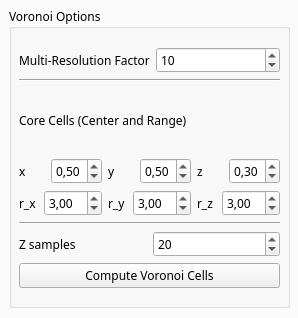
\includegraphics[width=0.28\linewidth]{Results/VoronoiOptions.png}
    }
    \hspace{20pt}
    \subfigure[Terrain dimensions section]{\label{fig:heightfieldDimensions}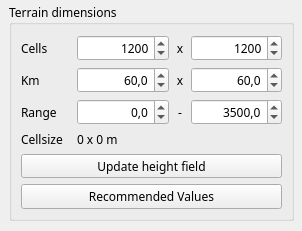
\includegraphics[width=0.35\linewidth]{Results/heightFieldSizes.png}
        }
    
    \caption{Voronoi options and Terrain dimensions windows of our applicaiton.
    Both windows can control the results of the decomposition}
    \label{fig:voronoiOptionsGeneral}
\end{figure}

\vspace{10pt}

Second, the user can also determine the generation of core cells (that will not be eroded
during the erosion algorithm). A rectangular block of core cells is 
always generated at a set position with a fixed size both specified by the user. The three parameters $(x,y,z)$ are numbers in 
the range $[0,1]$ and define the \textit{center} of the core cell block. The parameters 
are normalized using the bounding box of the terrain, so $(0.5, 0.5, 0.5)$ 
represents the center of the box. Next, $(r_x, r_y, r_z)$ define 
the \textit{range} of the core cell block. In order to normalize those 
values, they measure the range in \textit{cell sizes}; that is, $r_x = 2$
represents a value of 2 times the size of a grid cell in the x dimension.
When performing operations with the bounding box of the terrain, keep 
in mind that the bounding box of the decomposition extends a little 
bit beyond the highest peak in the $z$ direction so that we can take samples 
outside of the terrain.

\begin{figure}
    \centering

    \subfigure[Core cells when using center $(0.2,0.2,0.1)$ and 
    range $(1,1,1)$]{\label{fig:coreCells02_02_01_1}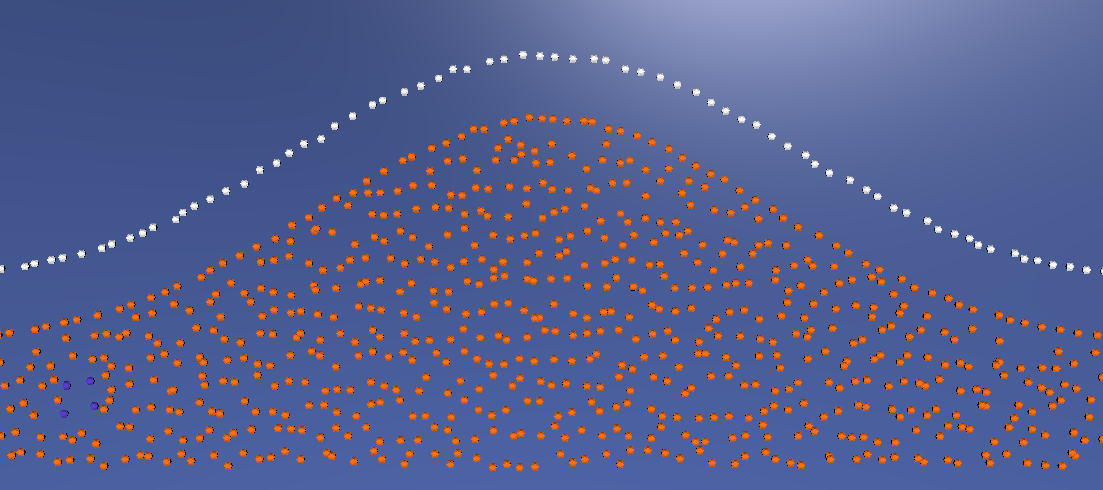
\includegraphics[width=0.45\linewidth]{Results/coreCells_02_02_01_1.png}
    }
    \hspace{20pt}    
    \subfigure[Core cells when using center $(0.8,0.8,0.1)$ and 
    range $(3,3,3)$]{\label{fig:coreCells08_08_08_3}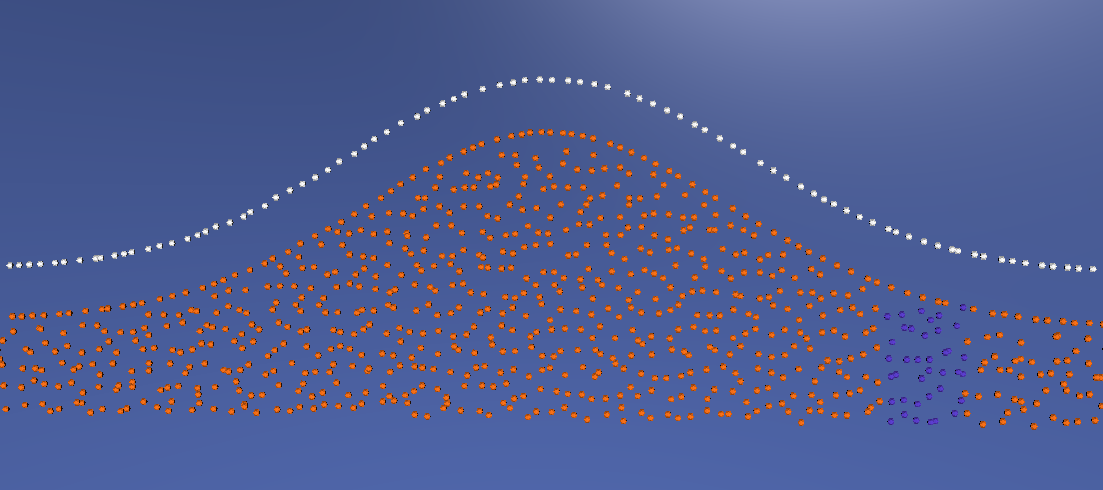
\includegraphics[width=0.45\linewidth]{Results/coreCells_08_08_01_3_2_3.png}}
    
    \caption{Results of modifying the parameters controlling the core 
    cell generation. Particles in purple represent core cells. Figure 
    taken using the \textit{Gaussian Bump} toy heightfield}
    \label{fig:voronoiCoreCells}
\end{figure}

\vspace{10pt}

Finally, the user has two options to modify the number of samples of the 
decomposition. The \textit{Terrain Dimensions} section 
on the left side of the UI (figure \ref{fig:heightfieldDimensions}) 
allows the user to modify the size of the heightfield. Because 
we are taking multiple samples for each cell of the heightfield, modifying 
the terrain dimensions will also modify the number of samples taken. 
Additionally, in the \textit{Voronoi Options} section, we can 
modify the \textit{zSamples} value, which will modify the number 
of vertical blocks of the 3D grid we construct to sample points.
As a final note, there is a button in the \textit{Terrain Dimensions} 
section called \textit{Recommended Values} that, for bigger terrains, 
will cap the dimensions (maintaining aspect ration) so they are feasible 
to compute. 

\begin{figure}
    \centering

    \subfigure[Salenques mountain sampled using a 256x184 grid (with 20 vertical samples)]{\label{fig:salenques256x184}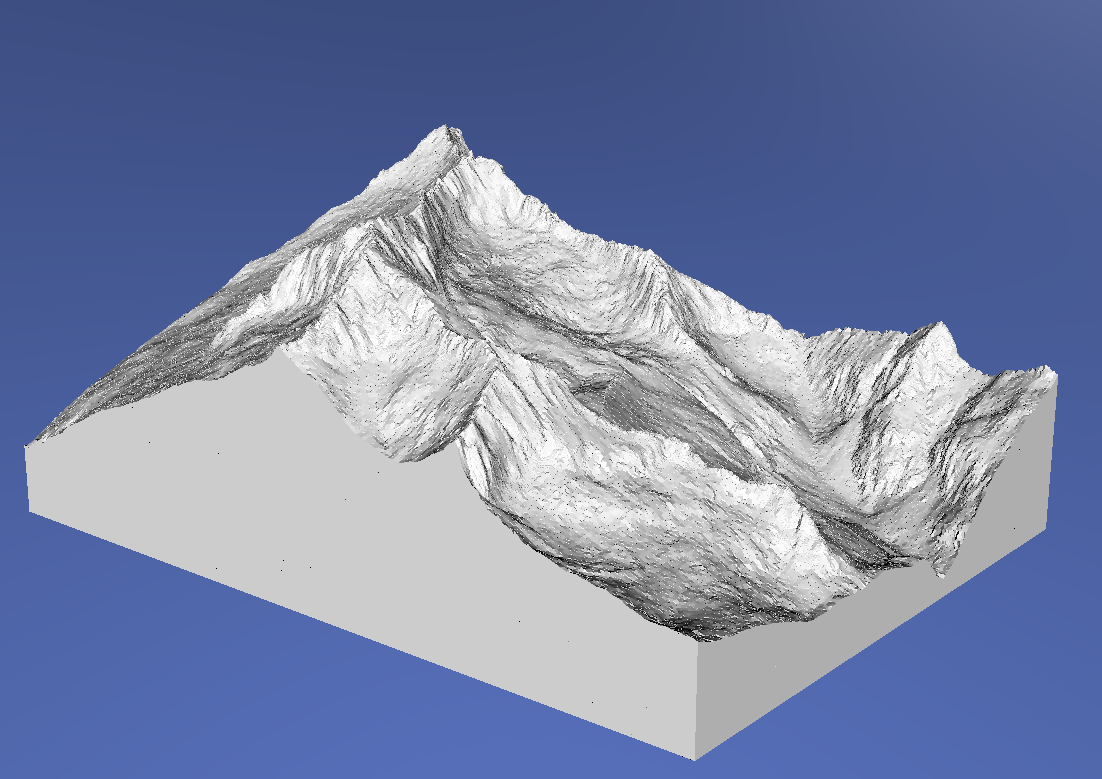
\includegraphics[width=0.4\linewidth]{Results/salenques256x184.png}
    }
    \hspace{20pt}    
    \subfigure[Salenques mountain sampled using a 64x46 grid (with 20 vertical samples)]{\label{fig:salenques64x46}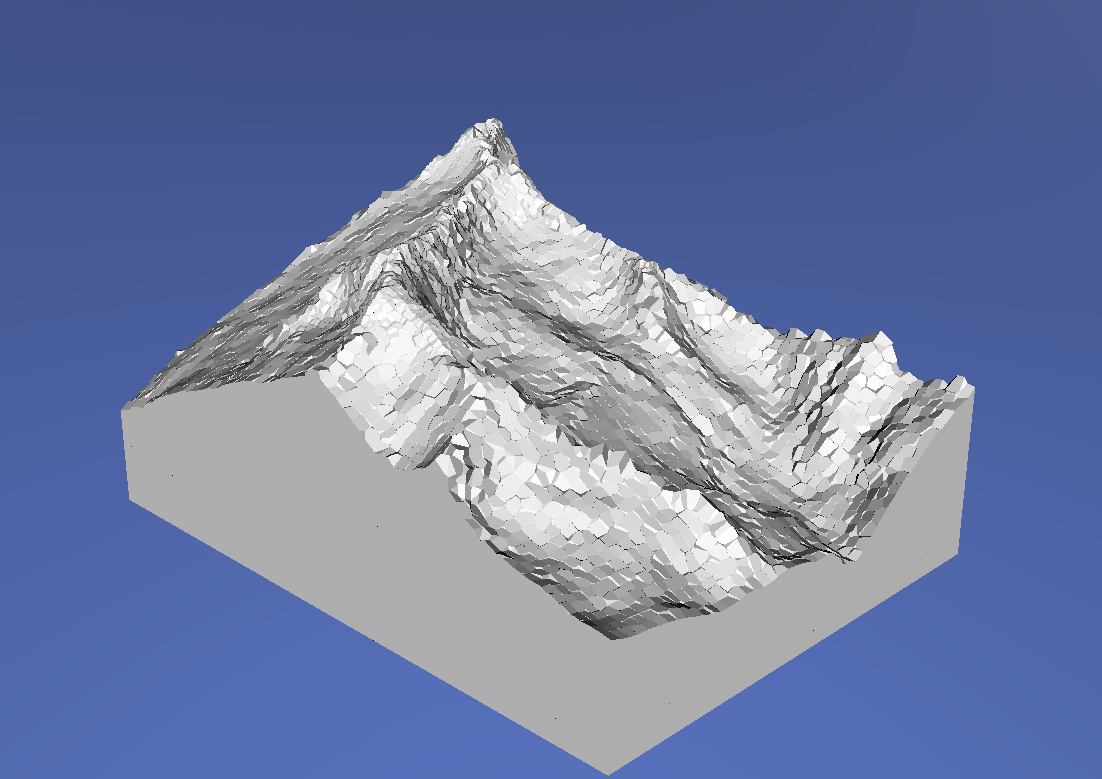
\includegraphics[width=0.4\linewidth]{Results/salenques64x46.png}}
    
    \caption{Results of modifying the heightfield dimensions on the terrain 
    Salenques}
    \label{fig:salenquesDimensionChange}
\end{figure}

\subsubsection{Visualization Options}

\begin{figure}
    \centering
    
    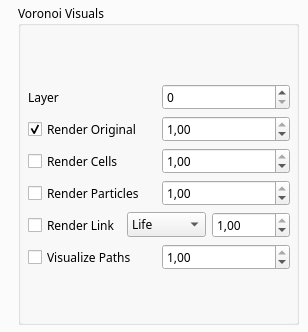
\includegraphics[scale=0.5]{Results/VoronoiVisuals.png}
    \caption{Voronoi Visuals section of the UI options}
    \label{fig:vorovisuals}
\end{figure}

In addition to the decomposition options, we also provided some options  
to visualize the results of said decomposition. Just above the 
\textit{Voronoi Options} section, there is a \textit{Voronoi Visuals} 
section (figure \ref{fig:vorovisuals}). Using these options we can 
visualize the original surface of the terrain, the decomposed terrain
made of cells, a visualization of the particles used to make the voronoi cells,
a visualization of the connections between cells (and their state, which 
will be useful when debugging the erosion simulation part), and a visualization 
of most recently generated water paths (also useful for the erosion 
part). The user can select multiple options to view multiple representations
simultaniously (like visualizing the original surface along other things, 
as seen in figure \ref{fig:particlesVsLinks}), and there is a variable 
next to each render option to modfiy the opacity of each of them. 

\begin{figure}
    \centering

    \subfigure[Example of the particle rendering mode]{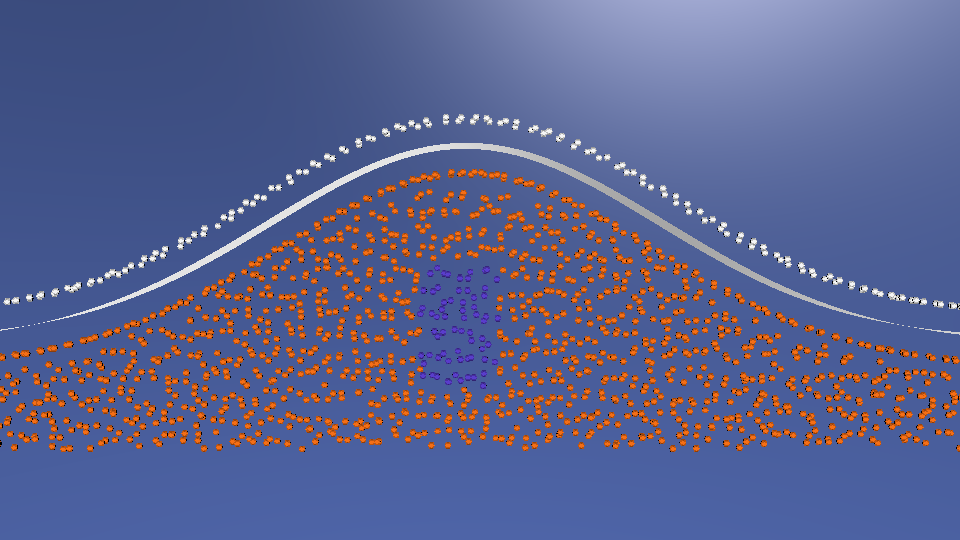
\includegraphics[width=0.35\linewidth]{Results/gaussianParticles.png}
    }
    \hspace{20pt}    
    \subfigure[Example of link rendering]{\label{fig:linksViz}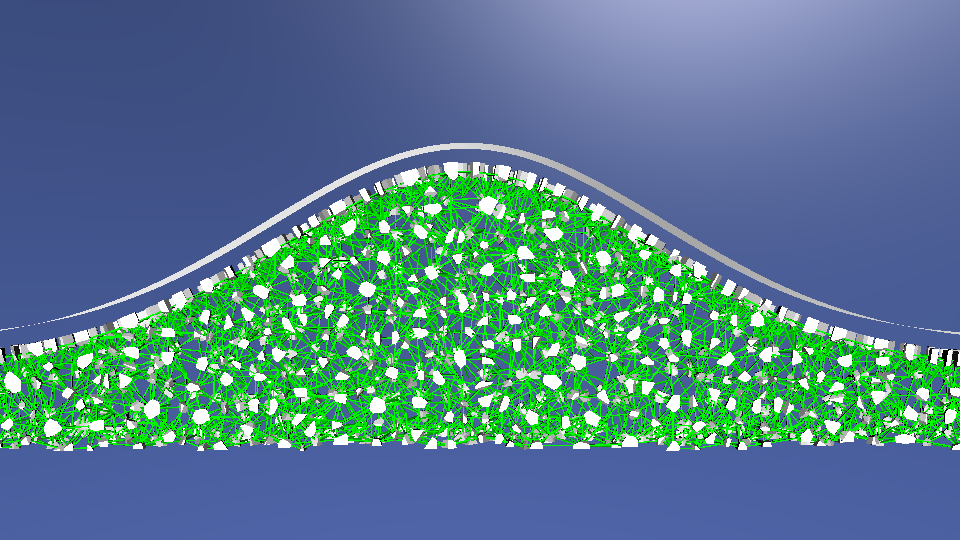
\includegraphics[width=0.35\linewidth]{Results/gaussianLinks.png}}
    
    \caption{Examples of diverse rendering options of our application. }
    \label{fig:particlesVsLinks}
\end{figure}


\subsection{Decomposition and Sampling Size Analysis}
In order to analyze our decomposition method, we performed multiple 
experiments varying the sampling size and the sampling method 
used to create the decomposition. By doing these tests, our 
intention was to better understand the relationship between 
the computational cost and the quality of the results, as well 
as to tune the parameters to obtain a good balance 
between cost and quality.

\vspace{10pt}

\subsubsection{Heightfield Dimensions Experiment}
Our first experiment tested the relationship between the heightfield 
dimensions (the base 2D grid) and the final results, both in terms of 
computation time and visual appearance. For this experiment we disabled
the cell subdivision protocol for high-rugosity cells, as changing 
the terrain dimensions might also have an effect on the rugosity, and 
we wanted to guarantee that the only changes to the model were the heightfield
dimensions. We also only used the terrain \textit{Punta Alta}, to avoid 
encountering differences between terrains.

\vspace{10pt}

We tried multiple sizes, and the results of the minimum, maximum and median 
tested dimensions can be appreciated in figure \ref{fig:2DdimensionResults}.
The terrain sampled using a 50x50 is really different from the other two, 
but the 200x200 does not have that much difference with the highest 
resolution tested, so it provides a good trade-off between efficiency and 
quality. 

\begin{figure}
    \centering

    \subfigure[Punta alta using a 50x50 grid]{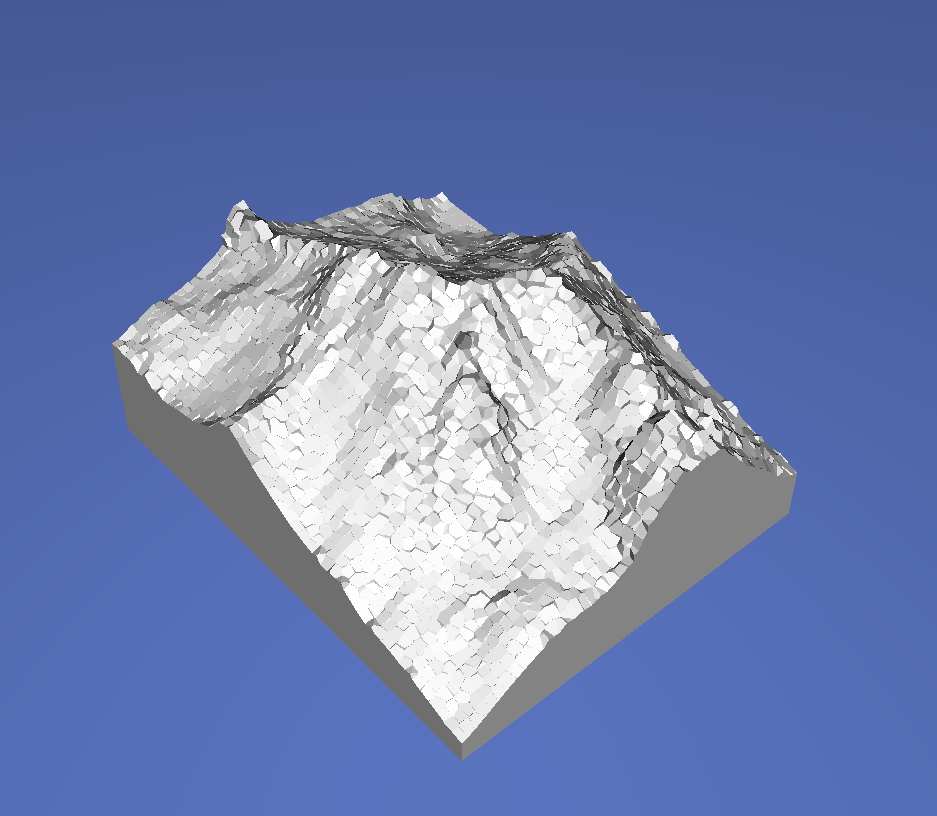
\includegraphics[width=0.3\linewidth]{Results/timeResults2D/puntaAlta50x50.png}
    }
    \hspace{10pt}    
    \subfigure[Punta alta using a 200x200 grid]{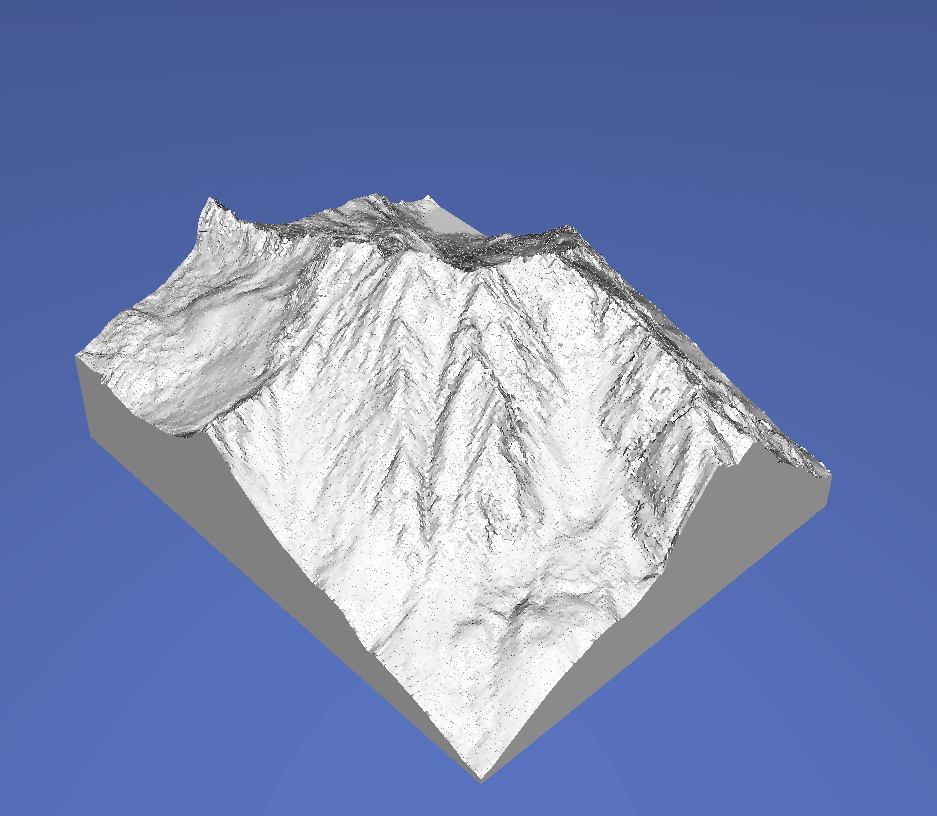
\includegraphics[width=0.3\linewidth]{Results/timeResults2D/puntaAlta200x200.png}}
    \hspace{10pt}
    \subfigure[Punta alta using a 350x350 grid]{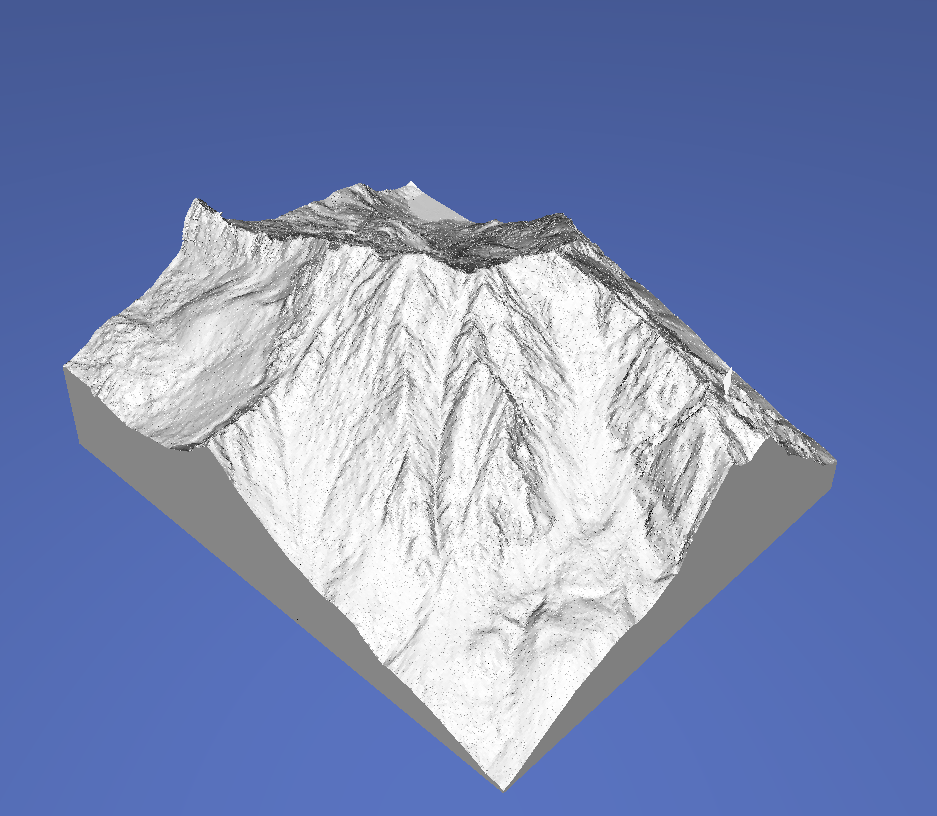
\includegraphics[width=0.3\linewidth]{Results/timeResults2D/puntaAlta350x350.png}}

    \caption{Results of modifying the heightfield dimensions in the terrain 
    Punta Alta}
    \label{fig:2DdimensionResults}
\end{figure}

\vspace{10pt}

Regarding the computational cost, if we consider a square heightfield NxN,
the number of particles generated is, of course, $O(N^2)$; however, the 
computation time is not as easy to determine. In the worst-case scenario,
computing a voronoi cell requires intersecting one plane for every other 
particle, so the computational cost would be $O(N^3)$. In practice, the library
voro++ \cite{osti_code-54674} implements this very efficiently, so this 
high theoretical cost might not appear in practice. In our empirical test, 
we found that the number of particles increased quadratically with 
the dimension $N$, but we also found that the time spent per particle 
also increased when increasing dimensions, so we can conclude that the 
relationship between number of particles and time is not fully linear.
These results can be seen in figure \ref{fig:2DtimeResults}. As a final note,
keep in mind that some aspects of the sampling depend on the terrain; as we 
avoid sampling outside the terrain, the number of samples in the z 
direction changes depending on the coordinates $(x,y)$, and the number 
of particles is not just $kN^2$ with $k$ representing the number of 
samples in the z direction.

\begin{figure}
    \centering

    \subfigure[Number of Dimensions vs Number of Particles]{
\includegraphics[width=0.35\linewidth]{Results/timeResults2D/dimensionParticles.png}
    }
    \hspace{20pt}    
    \subfigure[Number of Dimensions vs Time spent per Particle]{
\includegraphics[width=0.35\linewidth]{Results/timeResults2D/timePerParticle.png}}
    
    \caption{Results of modifying the heightfield dimensions in the terrain 
    Punta Alta on computation time}
    \label{fig:2DtimeResults}
\end{figure}

\subsubsection{Changing the Samples in the z-direction}

So far, we have only changed the dimensions of the heightfield, which is a 
2D grid. However, we sample points on a 3D grid, defined by the 
heightfield dimensions and the variable \textit{zSamples}. We also
experimented with this variable, and the results have been a 
bit surprising. The main factor of the visual quality of 
the decomposition is the accuracy at the surface, as anything below 
that cannot be seen until we perform erosion, which implies that 
increasing the number of samples in the z direction would be 
initially unappreciable (as seen in figure \ref{fig:zSamples10v99}). 
 

\begin{figure}
    \centering

    \subfigure[Results using $zSamples = 10$]{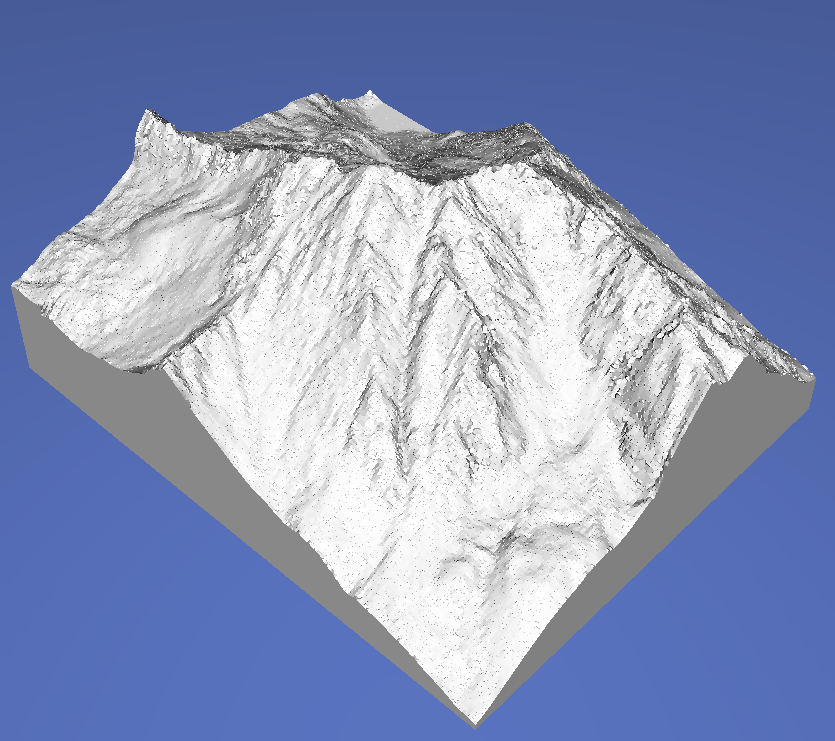
\includegraphics[width=0.3\linewidth]{Results/timeResultsZ/z10.png}
    }
    \hspace{20pt}    
    \subfigure[Results using $zSamples = 99$]{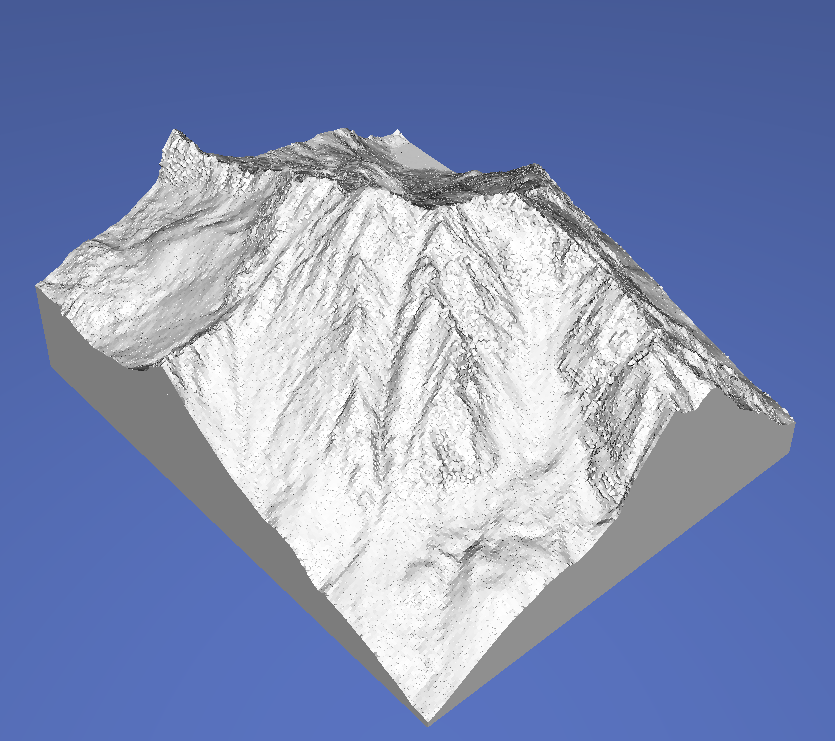
\includegraphics[width=0.3\linewidth]{Results/timeResultsZ/z99.png}}
    
    \caption{Results of modifying the variable $zSamples$ on the terrain 
    Punta Alta}
    \label{fig:zSamples10v99}
\end{figure}

\vspace{10pt}

The negligible effect on visual results was expected, but the unexpected 
part comes from the time spent to perform the decomposition. From the 
results that we got trying different values of $zSamples$, we extracted 
the time spent per particle, and we observed that this value decreases 
as the number of samples in the z direction increases (and thus 
the number of particles), which is exactly the opposite of what happened
when increasing the dimensions of the heightfield. We hypothesise 
that the particles on the surface are the ones with more computational 
cost, so increasing the number of samples in the z direction reduces 
the proportion of particles with high complexity, decreasing the 
average cost per particle.


\begin{figure}
    \centering
    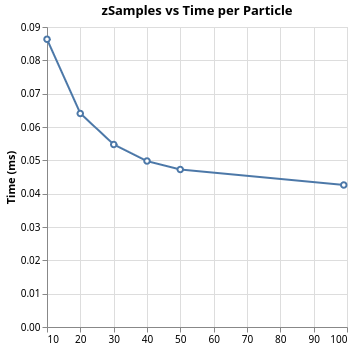
\includegraphics[scale=0.5]{Results/timeResultsZ/zSamplesTimePerParticle.png}
    \caption{Number of samples in the z direction vs computation time 
    spent per particle}
\end{figure}

\subsubsection{Experimenting with Rugosity Thresholds}

For our final test of the terrain decomposition, we reactivated the 
cell subdivision, and we experimented with different rugosity thresholds 
for subdivisions. First, we tested only performing one subdivision and changing 
the rugosity threshold (all rugosities are measured using a window 
size of $8$). The results of this experiment can be seen in figure 
\ref{fig:rugosityResults1}.


\begin{figure}
    \centering

    \subfigure[Bassiero terrain using a 151x138 grid. Subdivision performed 
    for cells with rugosity $> 1.5$]{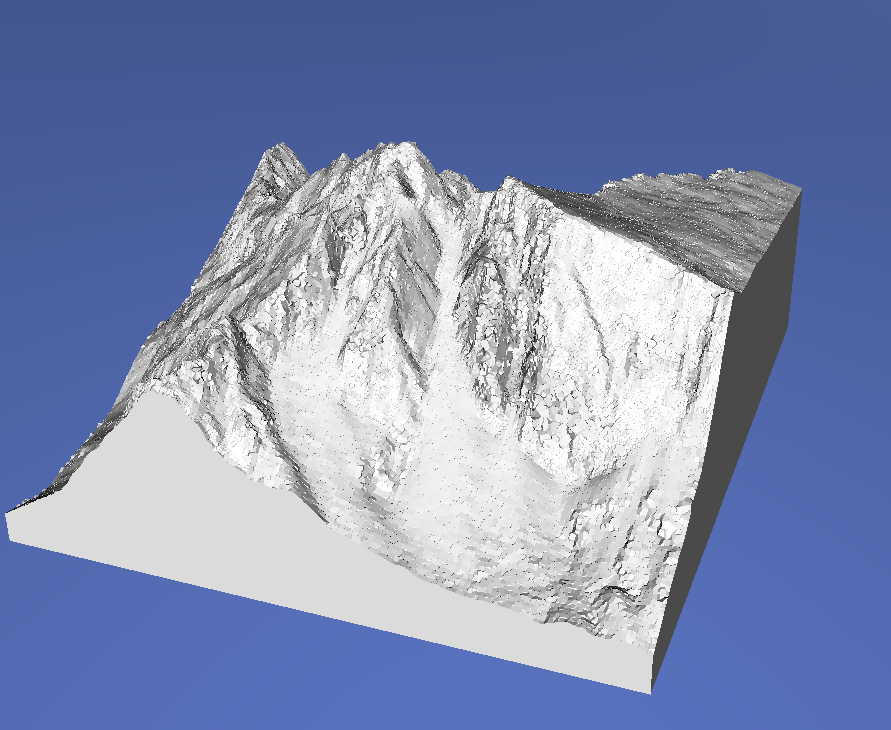
\includegraphics[width=0.3\linewidth]{Results/rugosityResults/division1.5.png}
    }
    \hspace{10pt}    
    \subfigure[Bassiero terrain using a 151x138 grid. Subdivision performed 
    for cells with rugosity $> 2.0$]{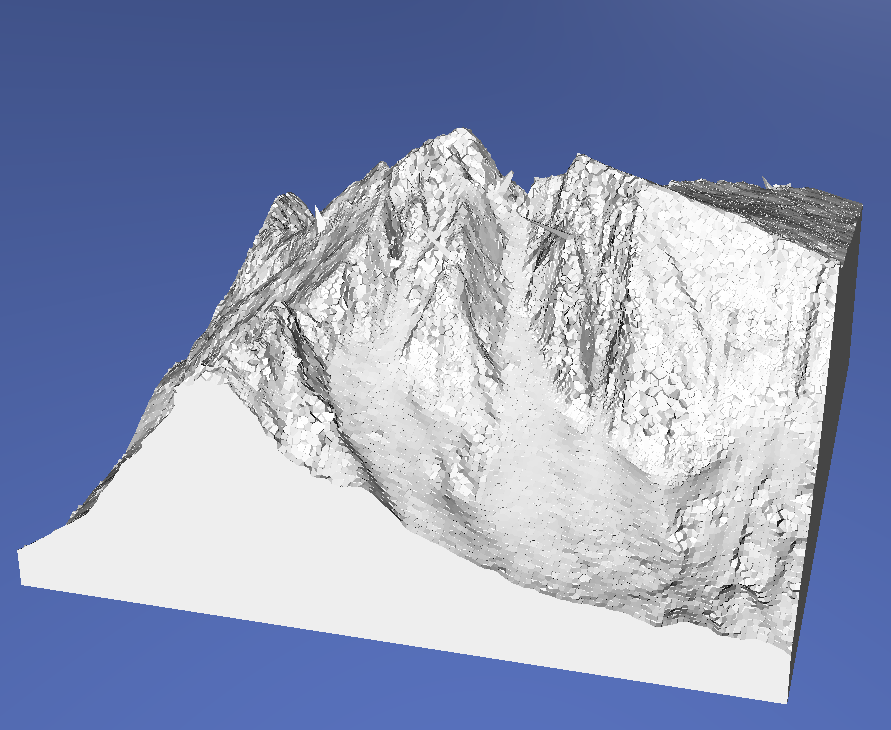
\includegraphics[width=0.3\linewidth]{Results/rugosityResults/divison2.0.png}}
    \hspace{10pt}
    \subfigure[Bassiero terrain using a 151x138 grid.Subdivision performed 
    for cells with rugosity $> 3.0$]{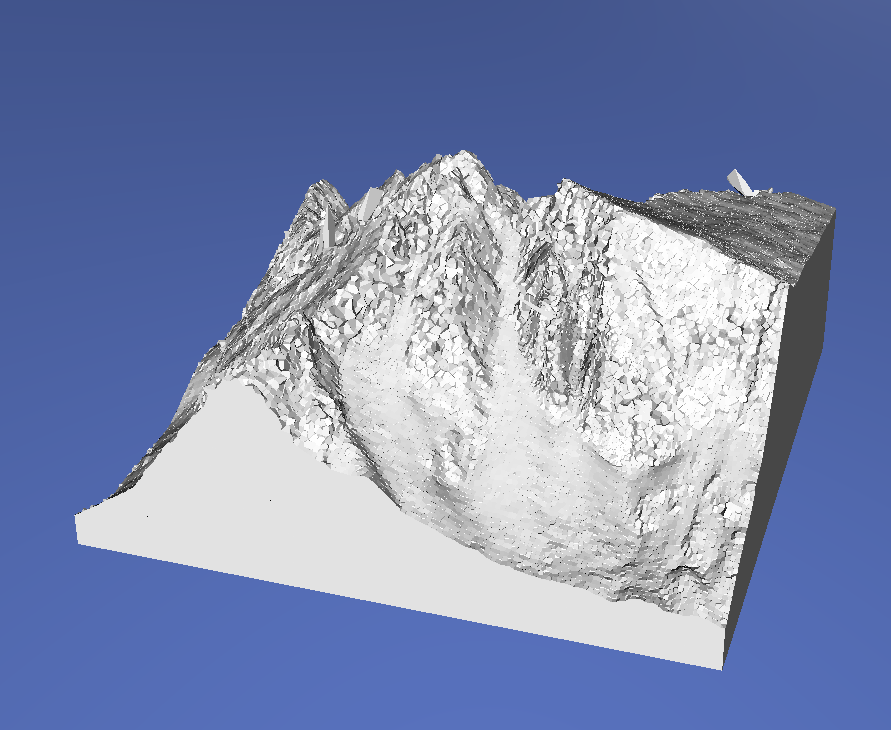
\includegraphics[width=0.3\linewidth]{Results/rugosityResults/division3.0.png}}

    \caption{Results of changing the rugosity threshold on the  
    Bassiero terrain} 
    \label{fig:rugosityResults1}
\end{figure}

\vspace{10pt}

Then, because we are not limited to subdividing a cell only once, we 
tried setting two or even three subdivision thresholds. This 
implies that we will collect $2 \cdot 4^k$ samples per cell at the surface, where 
$k$ is the number of thresholds surpassed on that specific cell. In this 
test we tried setting the threshold combinations $\{1.5,2.0\}$ (the one 
definitively implemented in the application), $\{2.0, 2.5\}$ and $\{1.5, 
2.0, 2.5\}$. There is a marked difference between the first and the 
second test, while the difference between the first and the last 
(which is the one with the highest quality) is more subtle and only appreciated 
in the sections with higher rugosity. 
\begin{figure}
    \centering

    \subfigure[Bassiero terrain using a 151x138 grid. Subdivision performed 
    for cells with rugosity $> 1.5$ and further subdivision for cells above $2.0$]{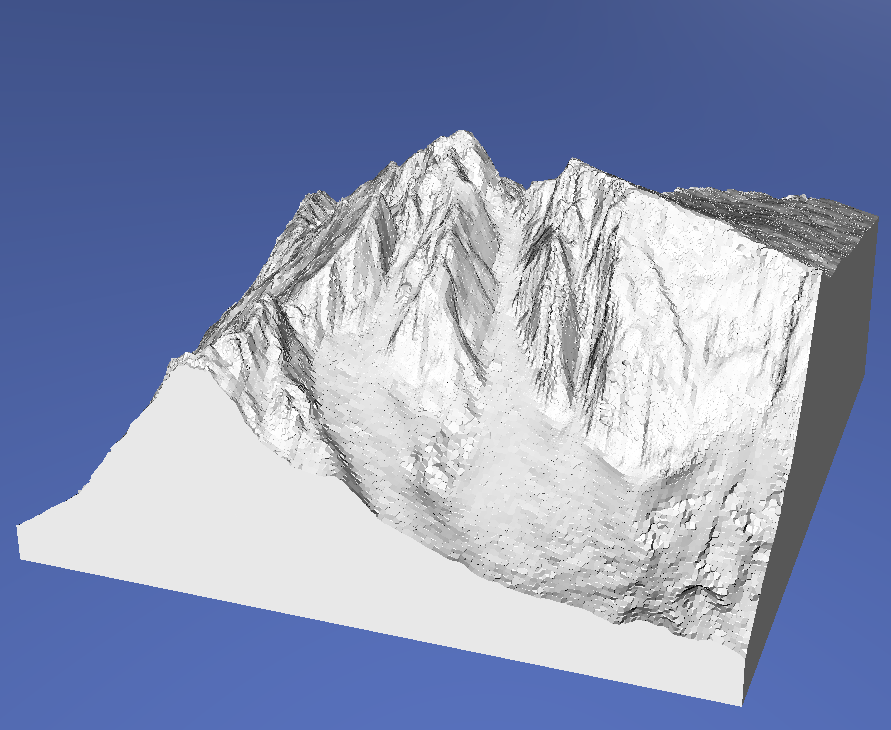
\includegraphics[width=0.3\linewidth]{Results/rugosityResults/division1.5_2.0.png}
    }
    \hspace{10pt}    
    \subfigure[Bassiero terrain using a 151x138 grid. Subdivision performed 
    for cells with rugosity $> 2.0$ and further subdivision for cells above $2.5$]{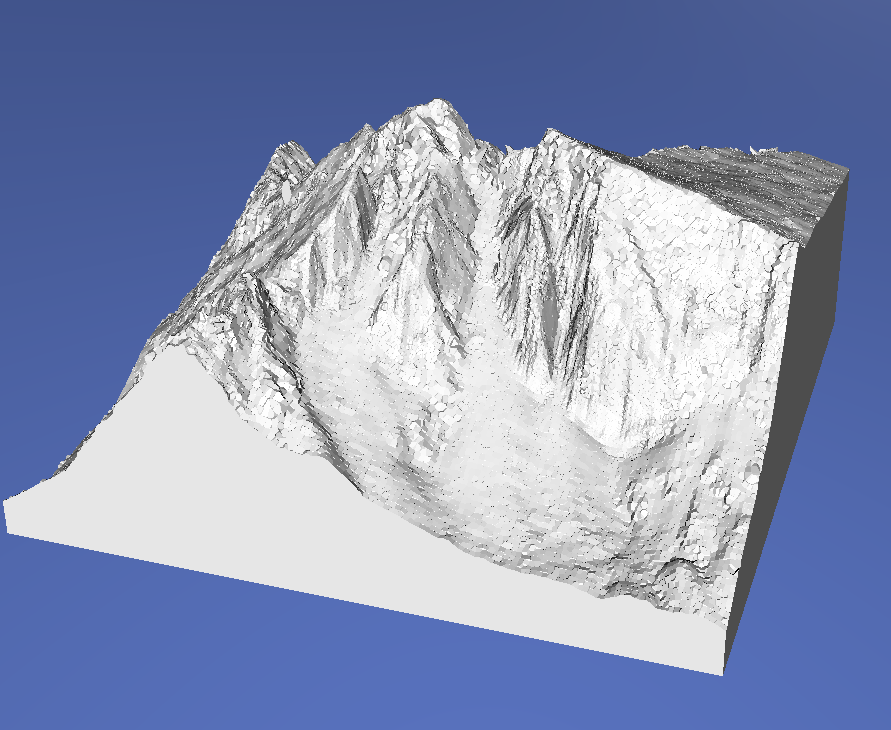
\includegraphics[width=0.3\linewidth]{Results/rugosityResults/division2.0_2.5.png}}
    \hspace{10pt}
    \subfigure[Bassiero terrain using a 151x138 grid.Subdivision performed 
    at three levels with thresholds $1.5$, $2.0$ and $2.5$]{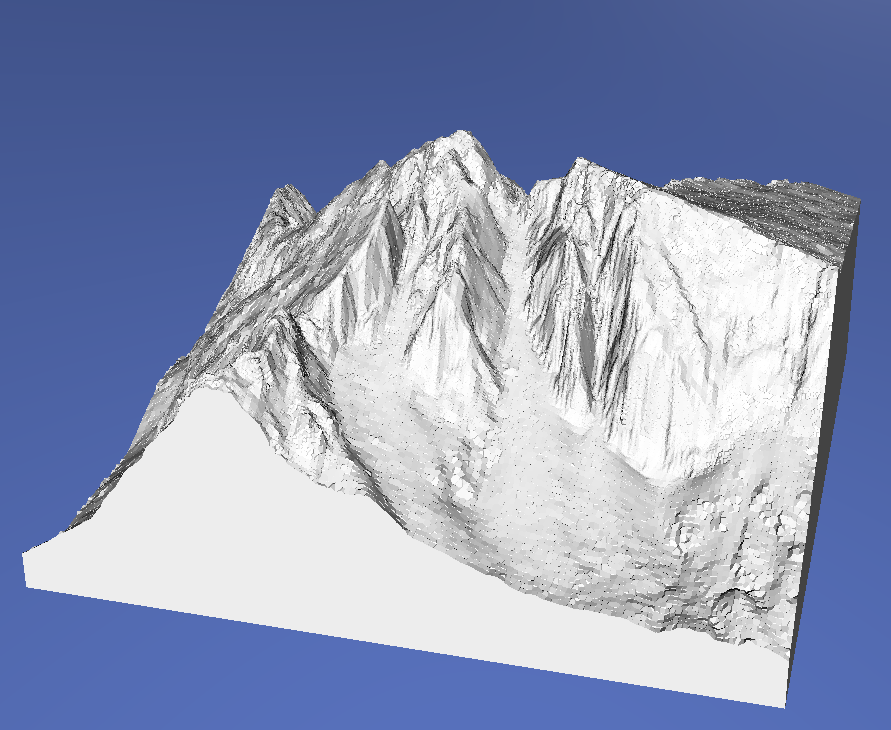
\includegraphics[width=0.3\linewidth]{Results/rugosityResults/division1.5_2.0_2.5.png}}

    \caption{Results of changing the rugosity threshold on the  
    Bassiero terrain. In this case, we performed further subdivisions 
    in cells where the rugosity is too high.} 
    \label{fig:rugosityResults2}
\end{figure}

\vspace{10pt}

Finally, we also measured the number of samples generated for every 
test, as well as its computation time. Table \ref{tab:rugosity} shows 
all measures we have taken for this batch of experiments. Remember 
that the computation time is not linear with respect to the number 
of particles, so it is important to choose a good balance between 
time spent and visual quality. In the final application, 
we decided to fix the threshold combination at $\{1.5, 2.0\}$, as 
we found that it provides a good balance.

\begin{table}[]
\centering
\begin{tabular}{|l|l|l|}
\hline
Thresholds             & Particles Generated & Time (s) \\ \hline
Base (No subdivisions) & 231713              & 12.639     \\ \hline
1.5                    & 293204              & 16.719     \\ \hline
2.0                    & 255445              & 14.180     \\ \hline
3.0                    & 233918              & 12.844     \\ \hline
1.5 \& 2.0              & 388023              & 22.715     \\ \hline
2.0 \& 2.5              & 285736              & 16.147     \\ \hline
1.5 \& 2.0 \& 2.5        & 509009              & 32.446     \\ \hline
\end{tabular}
\caption{Measures of our tests with different rugosity thresholds}
\label{tab:rugosity}
\end{table}

\subsubsection{Different Lighting Test}
The lighting method that we use highlights the borders between cells, 
as each face has a different normal. The lighting method chosen is 
useful to debug, but it can reduce the visual quality in some situations. 
As an experiment, we decided to reuse the same lighting method used to render 
the base heightfield (the one that the base application used) to 
properly compare the base model with its decomposition. Figure \ref{fig:lightingTest}
shows the results of this experiment: the terrain looks basically the 
same except for the walls (generated during the decomposition). It is 
important to note that this lighting method assigns a color based 
on the position of a point in the 2D grid of the DEM, so all points 
with the same $(x,y)$ coordinates will have the same color.

\begin{figure}
    \centering

    \subfigure[Base Aneto terrain]{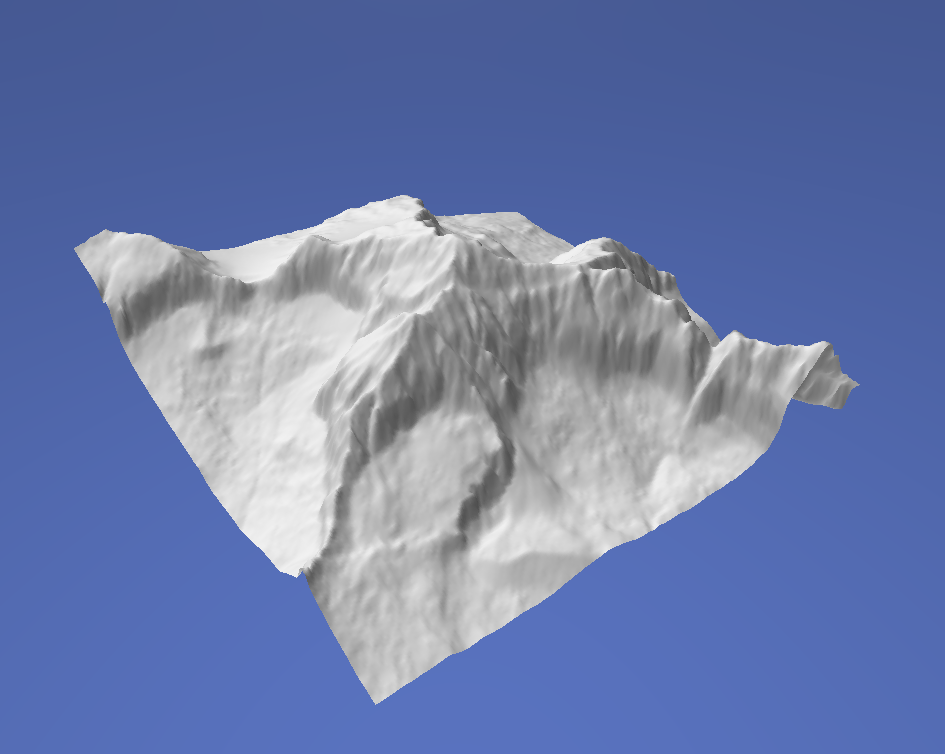
\includegraphics[width=0.4\linewidth]{Results/BaseAneto.png}
    }
    \hspace{20pt}    
    \subfigure[Aneto terrain after the decomposition]{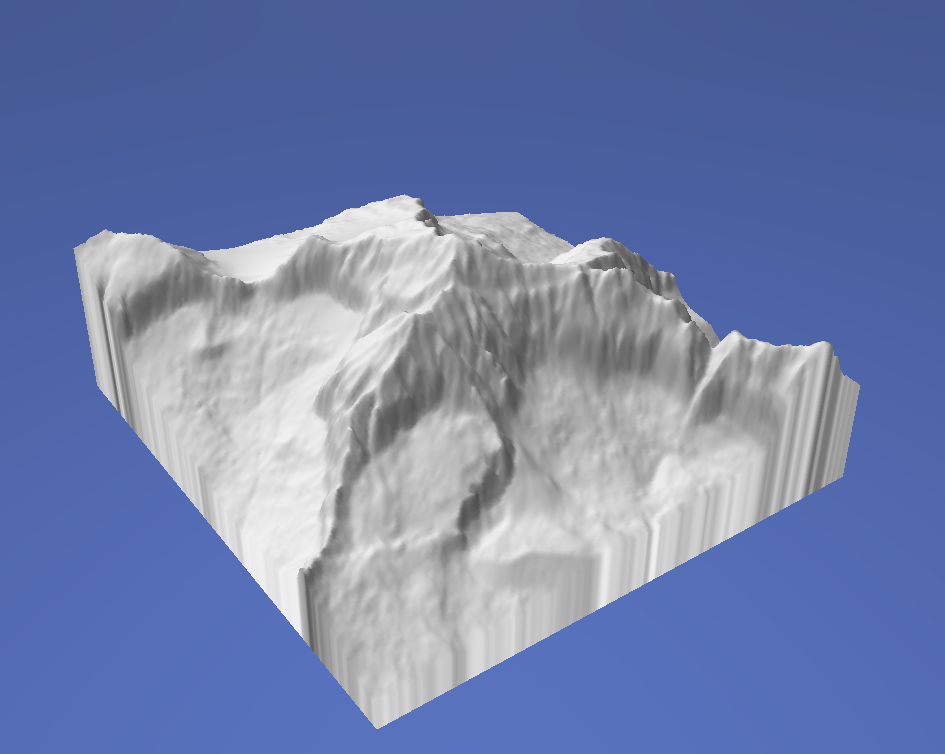
\includegraphics[width=0.4\linewidth]{Results/AnetoCells.png}}
  
    \caption{Comparison of the base terrain and the decomposition result using 
    the same lighting} 
    \label{fig:lightingTest}
\end{figure}

\subsection{Multi-Resolution Comparison}

In addition to the tests regarding the initial decomposition, we also 
compared our two proposed methods for subsampling. These two methods 
are hard to compare, as the method of subsampling in a grid does 
not allow for an easy manipulation of the total size of the subsampling 
(the grid that we use to sample and subsample is terrain dependent so 
we cannot know the exact size of the sampling). 
Despite these limitations, we decided to take some measures for each 
method in order to perform some comparisons. 

\vspace{10pt}

First, we tested both the time to compute and the final result of the 
furthest point sampling using $N/s$ subsamples where $s \in \{3,5,10,20\}$, 
and then, we tested the subsampling method based on a grid using 2x2x2, 
3x3x3, and 4x4x4 blocks of grid cells. The visual results can be appreciated 
in figures \ref{fig:furthestComparison} and \ref{fig:gridMultiRes}, and 
the computation time of each situation is written in table \ref{tab:subsamplingTable}.
All time measures are taken from the start of the decomposition to the 
completion of the low-resolution layer, so they all include the base time 
to produce the initial sampling. 

\vspace{10pt}

Even if these two methods are hard to compare, we can see that, 
with a similar amount of particles (using a downsampling factor of 
20 vs a 2x2x2 grid), the grid method is much more efficient in producing 
the computation and also produces shapes that more closely resemble 
the base terrain. Additionally, the examples that use the grid 
method add very little overhead over the initial sampling of the 
decomposition; if we subtracted the time of the initial computation 
to the total computation times, we would see a sharper difference 
between the furthest point and the grid methods. 

\begin{figure}
    \centering

    \subfigure[Bassiero terrain subsampled using furthest point with a downscale factor of $3$]{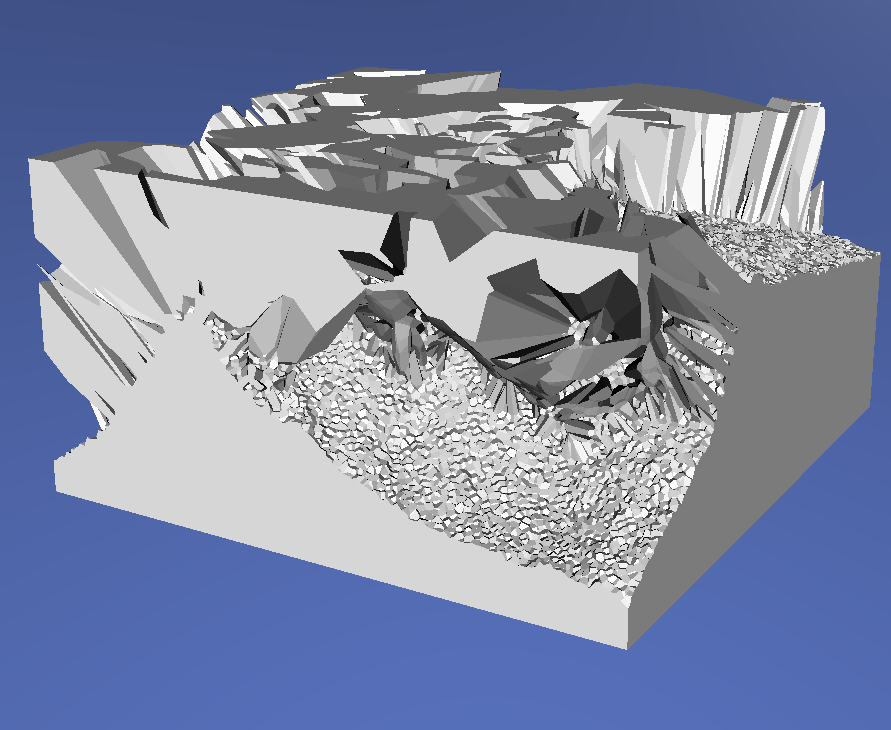
\includegraphics[width=0.3\linewidth]{Results/MultiResComparison/furthest3.png}
    }
    \hspace{10pt}    
    \subfigure[Bassiero terrain subsampled using furthest point with a downscale factor of $5$]{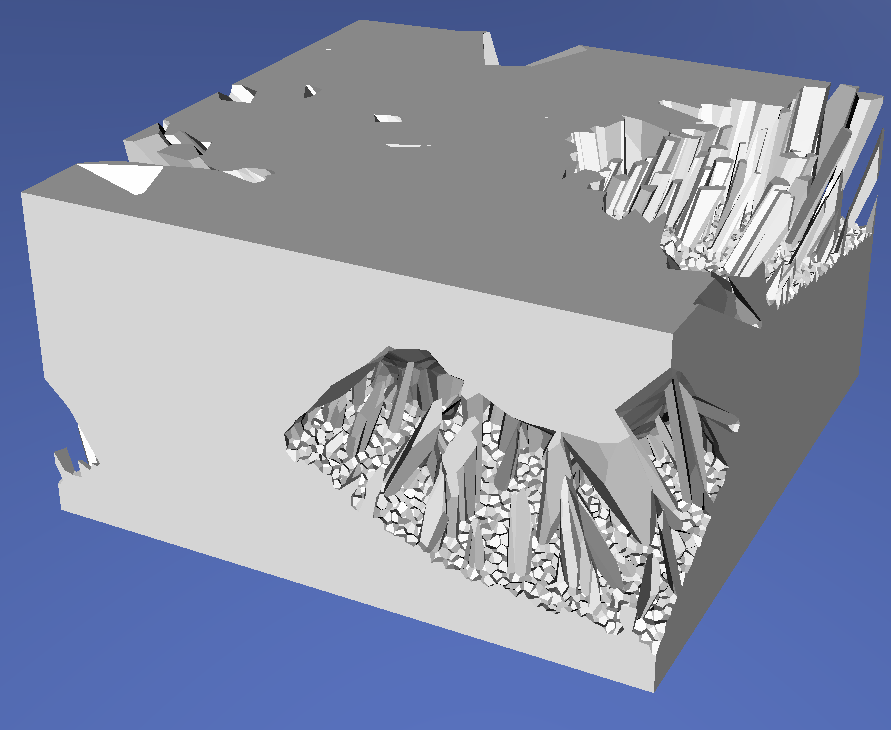
\includegraphics[width=0.3\linewidth]{Results/MultiResComparison/furthest5.png}}
    \hspace{10pt}
    \subfigure[Bassiero terrain subsampled using furthest point with a downscale factor of $10$]{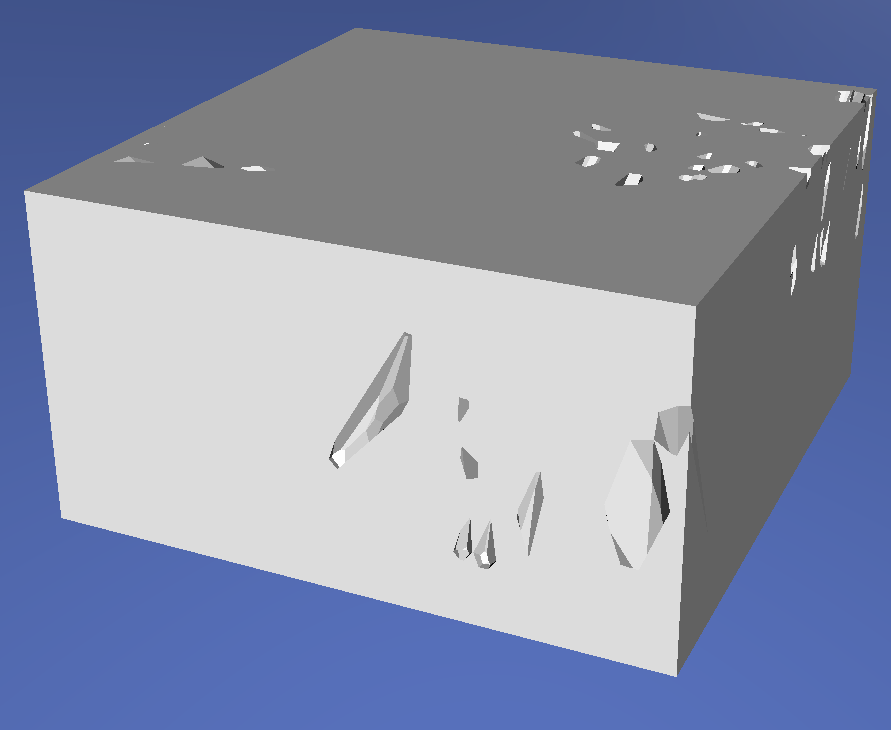
\includegraphics[width=0.3\linewidth]{Results/MultiResComparison/furthest10.png}}

    \caption{Different downscaling factors for the furthest point sampling method 
    applied to the \textit{Bassiero} terrain. 
    } 
    \label{fig:furthestComparison}
\end{figure}

\begin{figure}
    \centering

    \subfigure[Bassiero terrain subsampled using a subgrid made of 2x2x2 blocks]{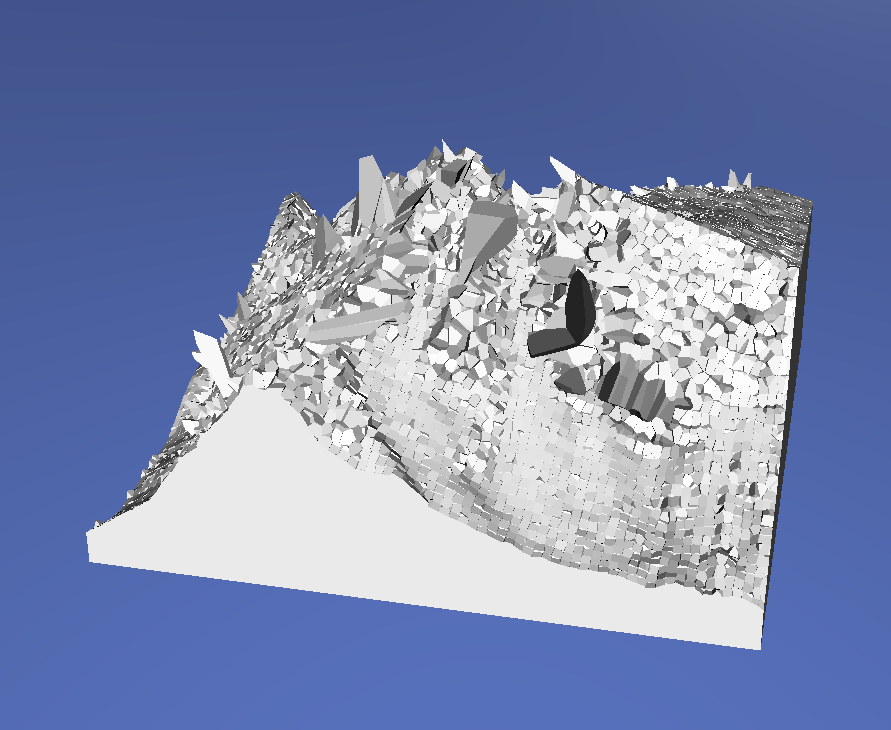
\includegraphics[width=0.3\linewidth]{Results/MultiResComparison/grid2x2.png}
    }
    \hspace{10pt}    
    \subfigure[Bassiero terrain subsampled using a subgrid made of 3x3x3 blocks]{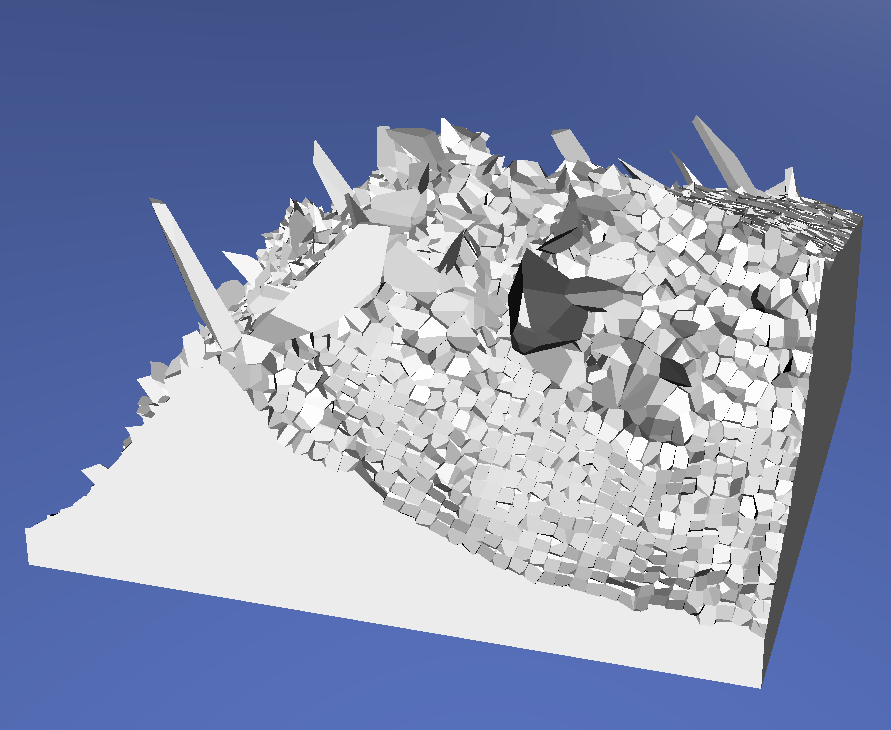
\includegraphics[width=0.3\linewidth]{Results/MultiResComparison/grid3x3.png}}
    \hspace{10pt}
    \subfigure[Bassiero terrain subsampled using a subgrid made of 4x4x4 blocks]{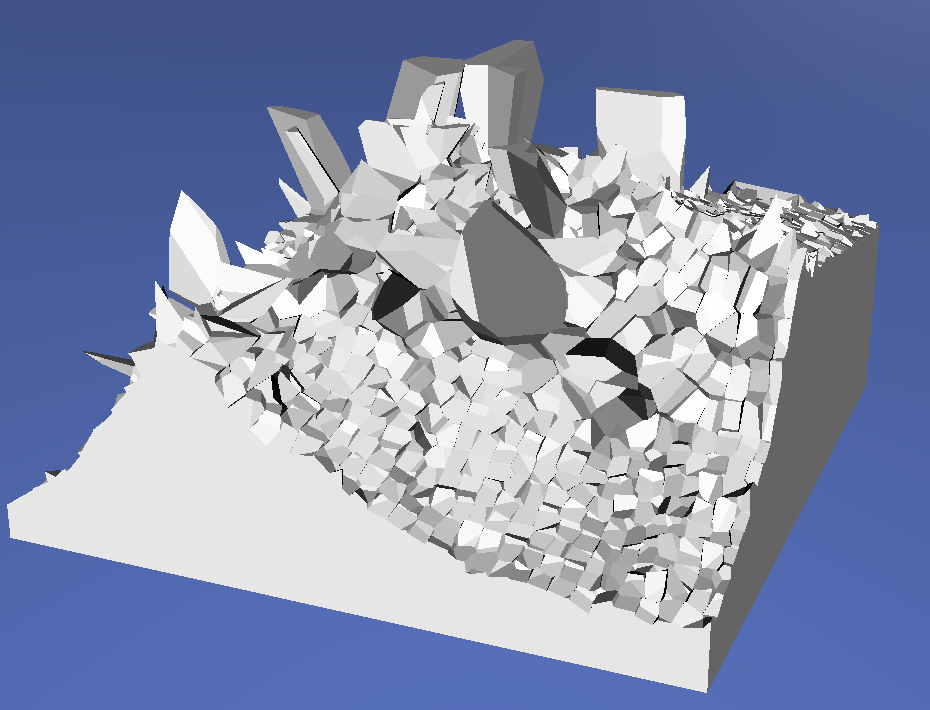
\includegraphics[width=0.3\linewidth]{Results/MultiResComparison/grid4x4.png}}

    \caption{Comparison of different block sizes used to make a subsampled gird. Applied to 
    the \textit{Bassiero} Terrain.} 
    \label{fig:gridMultiRes}
\end{figure}

\begin{table}[]
\centering

\begin{tabular}{|l|l|l|}
\hline
Multi-Resolution factor  & Particles Generated & Time (s) \\ \hline
Base (single resolution) & 411635              & 22.813     \\ \hline
Furthest Point: 3        & 137211              & 283.913    \\ \hline
Furthest Point: 5         & 82327               & 183.684    \\ \hline
Furthest Point: 10        & 41163               & 103.141    \\ \hline
Furthest Point: 20        & 20581               & 64.237     \\ \hline
Grid: 2x2x2              & 26208               & 25.673     \\ \hline
Grid: 3x3x3              & 10294               & 24.210     \\ \hline
Grid: 4x4x4              & 5398                & 23.775     \\ \hline
\end{tabular}
\caption{Comparison between the two subsampling methods that we implemented}
\label{tab:subsamplingTable}
\end{table}



\section{Erosion Simulation}
In this project we deeply tested the erosion simulation algorithm, trying 
different paramaters and different decompositions, comparing the old 
algorithm versus the new one. In this section we are going to go over 
our implementation of the erosion process as well as explain all our 
findings from our experiments.

\subsection{UI For Erosion}
Before explaining our findings, we are going to show how the user can 
control the different aspects of the simulation. Most parameters, 
like the material properties are set in the \textit{mechanicalModel.h} 
header with no option to control them on the UI, but the user still 
has some freedom using just the UI.

\subsubsection{Erosion Menu}

From the erosion menu of the UI (shown in figure \ref{fig:erosionMenu}), the 
user can modify the direction of water infiltration (as explained in section
\ref{sec:waterPaths}) and whether the mechanical model is used or not 
(keep in mind that an initial stress computation will be performed 
every time you activate the mechanical model option). 
Even if the user decides to not use the mechanical model, the button 
\textit{Compute Stresses} computes all stresses of the system and removes 
the links meeting the failure conditions; this way, we can simulate the 
process without the mechanical model up to a point and then compute all 
stresses of the system in that state. 

\vspace{10pt}

Finally, the user will have to select the number of paths to be generated 
simultaneously and press the button \textit{Compute Water Paths} to 
start the simulation.  
\begin{figure}
    \centering
    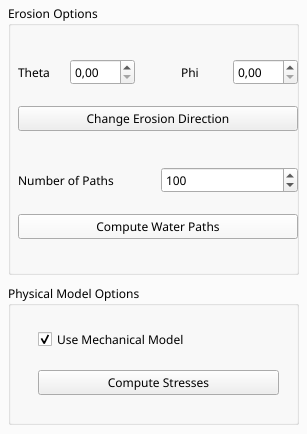
\includegraphics[scale=0.45]{Results/erosionMenu.png}
    \caption{Erosion menu of the UI}
    \label{fig:erosionMenu}
\end{figure}
\subsubsection{Visualization Options}
In addition to the simulation control options, the 
visualization menu \ref{fig:vorovisuals} also contains two options 
that are useful to debug the erosion process. First, we can visualize
the life of the links and their shear and normal stresses using 
the \textit{Render Links} option (figure \ref{fig:linkVisualization}), 
and second, we can paint blue the cells touched by the last batch of 
water paths (remember that the size of the batch is controlled using the 
erosion options), as shown in figure \ref{fig:waterPaths}.

\begin{figure}
    \centering

    \subfigure[Link life visualization. From Green (full life) to red (fully damaged)]{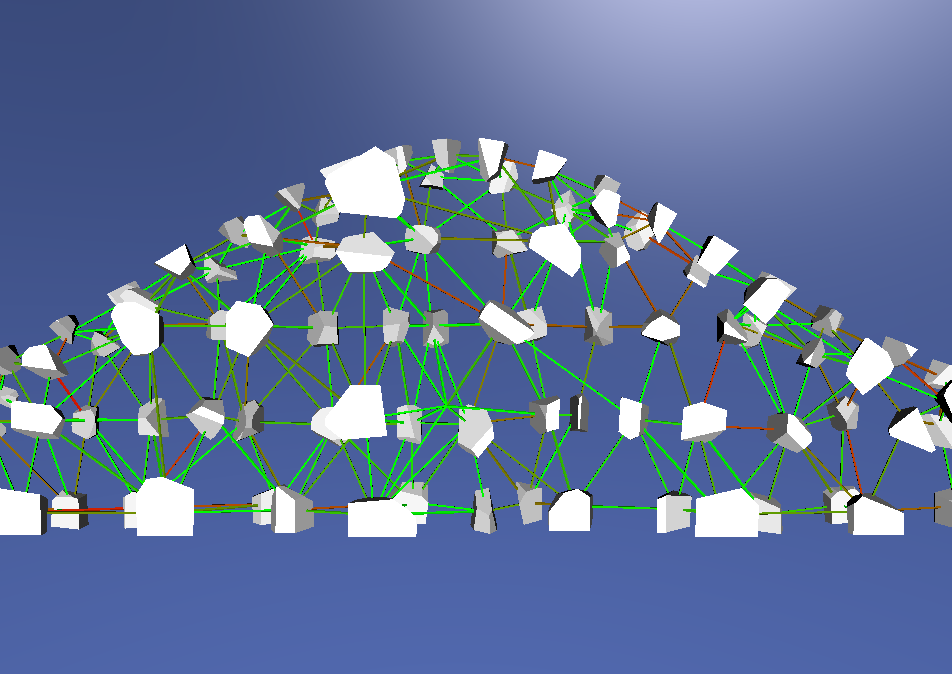
\includegraphics[width=0.278\linewidth]{Results/linkLife.png}
    }
    \hspace{10pt}    
    \subfigure[Link normal stress visualization. From blue to green for negative 
    normal stress (compression) and green to red for tension]{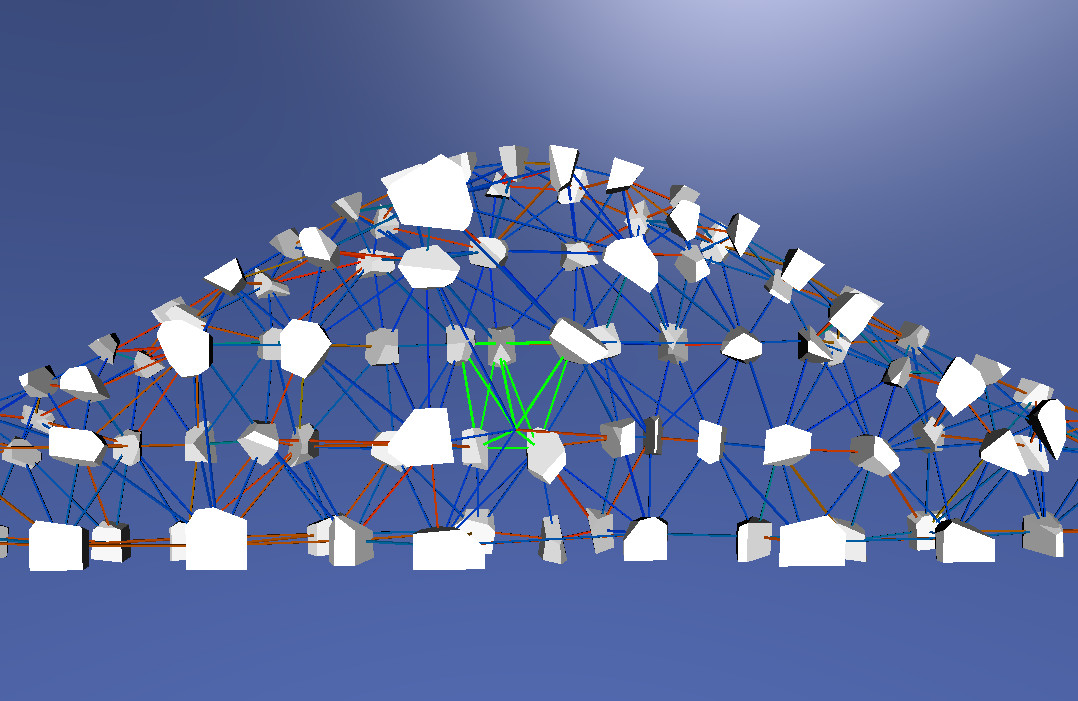
\includegraphics[width=0.3\linewidth]{Results/linkNormalStress.png}}
    \hspace{10pt}
    \subfigure[Link shear stress visualization. From green (0 stress) to red]{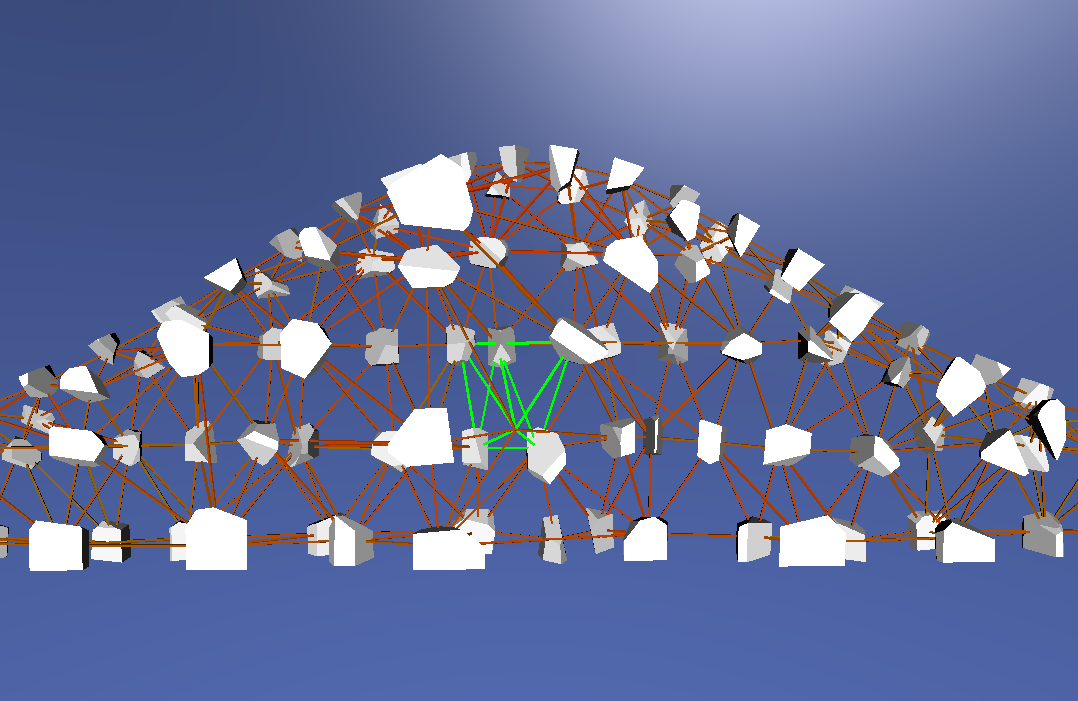
\includegraphics[width=0.3\linewidth]{Results/linkShearStres.png}}

    \caption{Different link visualization options} 
    \label{fig:linkVisualization}
\end{figure}

\begin{figure}
    \centering
    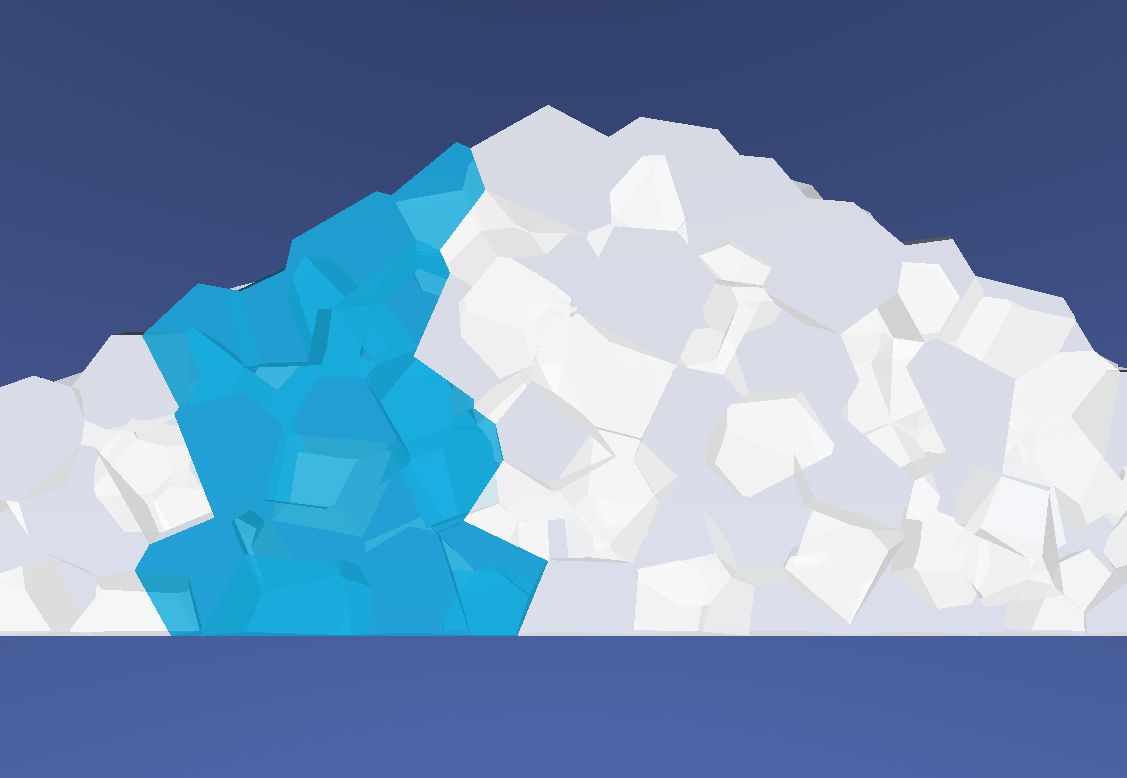
\includegraphics[scale=0.15]{Results/waterPaths.png}
    \caption{Simulation of 10 water paths on the \textit{Gaussian Bump}
    toy example. Cells that are touched by the water are painted in blue}
    \label{fig:waterPaths}
\end{figure}
\subsection{Base Algorithm Experimentation}
The first experiments that we conducted were all centered on 
the base algorithm as designed in \cite{10.2312:ceig.20241139}, without the inclusion of the mechanical model.
Having a set of experiments on the base method allows us to better 
compare both techniques and pinpoint the advantages of adding 
the mechanical model on top of the base one. 

\vspace{10pt}

Our first batch of experiments consited in comparing both 
implemented multi-resolution methods to check the difference 
in results and, additionally take measures of computational time. For 
these experiments, we tested 5 consecutive rounds of 10,000 paths for 
each multi-resolution method using the terrain \textit{Aneto} with 
resolution 197x199, and then 
3 consecutive rounds of 100,000 paths on a fresh instance of the 
same terrain. We decided to take multiple rounds of paths instead 
of just one single round with the combined number of paths to observe 
the evolution of the terrain step by step and check the influence 
of the current state of the terrain on the computational cost.

\vspace{10pt}

Regarding the final results, figure \ref{fig:100K Comparison} shows 
the base Aneto terrain compared against the result of simulating 
300 thousand water paths on each multi-resolution method. The 
furthest point method generated more cells than the grid method 
(66491 vs 18736), so a slower erosion process was expected. Still, 
as we mentioned in section \ref{sec:multiResolution}, the furthest 
point method has to consider some cells outside of the terrain 
as solid; this means that in order to start appreciating results on 
the terrain, we will have to wait for the outside cells to be removed, 
which makes the full simulation slower. 

\vspace{10pt}

In terms of the computational cost, we have seen that it increased 
for every consecutive round of 10,000 paths with both subsampling 
methods (figure \ref{fig:10KTime}). We think that the more damaged the 
links are, the more removal events will be triggered, which are the 
most computationally expensive procedures of the algorithm, so the total 
computation time will increase. Additionally, the more eroded the 
terrain is and the fewer cells remaining, the faster the algorithm 
should run, as the size of the problem becomes smaller. Following this logic, 
there should be a threshold where the cost of each consecutive round 
starts decreasing instead of increasing, as the size of the terrain 
starts getting significantly smaller.
Figure \ref{fig:100KTime} 
seems to confirm this idea, as the computational cost 
of the 100,000 path rounds decreases for each consecutive run 
in the grid method case. In the case of the furthest point sampling, 
we have already seen that the erosion process is slower, so we think 
that 300 thousand paths were not enough to reach the threshold where 
the time starts decreasing instead of increasing.


\begin{figure}
    \centering

    \subfigure[Aneto terrain before any erosion process]{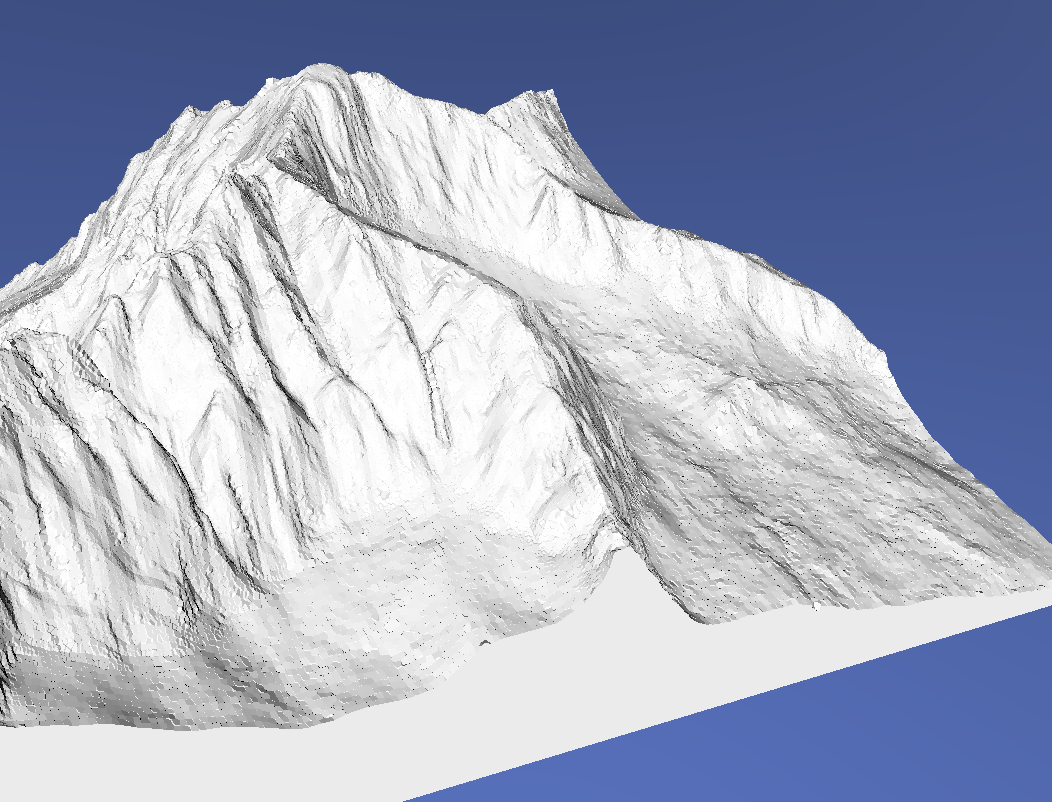
\includegraphics[width=0.3\linewidth]{Results/AnetoBefore300k.png}
    }
    \hspace{10pt}    
    \subfigure[Aneto terrain after 300 thousand paths using the furthest point method to subsample]{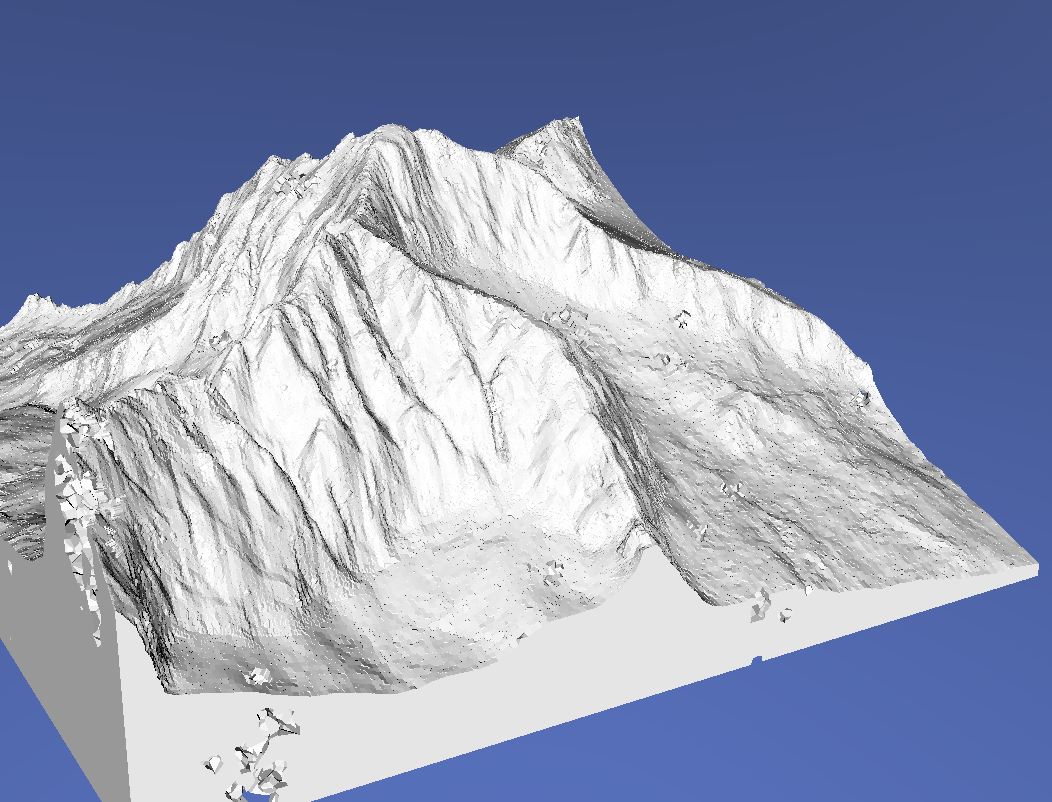
\includegraphics[width=0.3\linewidth]{Results/Aneto300K_general.png}}
    \hspace{10pt}
    \subfigure[Aneto terrain after 300 thousand paths using the grid method to subsample]{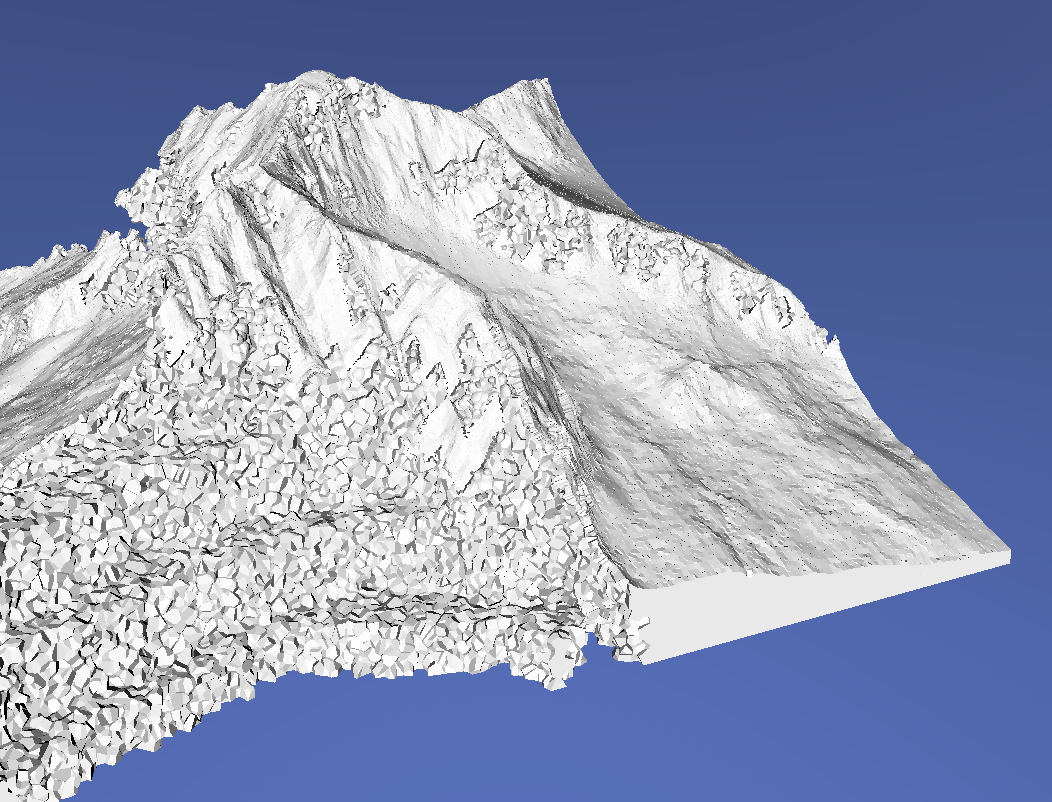
\includegraphics[width=0.3\linewidth]{Results/AnetoAfter300k.png}}

    \caption{Result of 300 thousand water paths on the Aneto terrain using different 
    subsampling methods to create the low-resolution decomposition} 
    \label{fig:100K Comparison}
\end{figure}

\begin{figure}
    \centering

    \subfigure[Time to complete different runs of 10K paths. The runs have been 
    executed one after the other on the same model]{\label{fig:10KTime}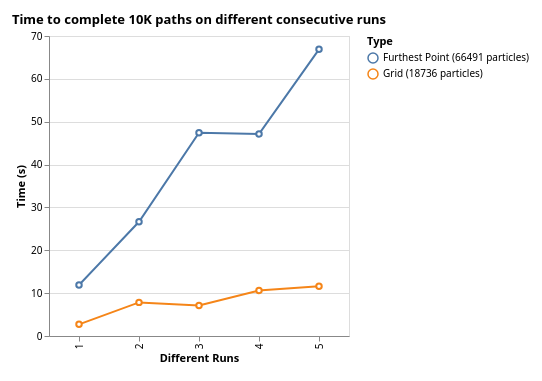
\includegraphics[width=0.4\linewidth]{Results/10KTime.png}
    }
    \hspace{20pt}    
    \subfigure[Time to complete different runs of 100K paths. The runs have been 
    executed one after the other on the same model]{\label{fig:100KTime}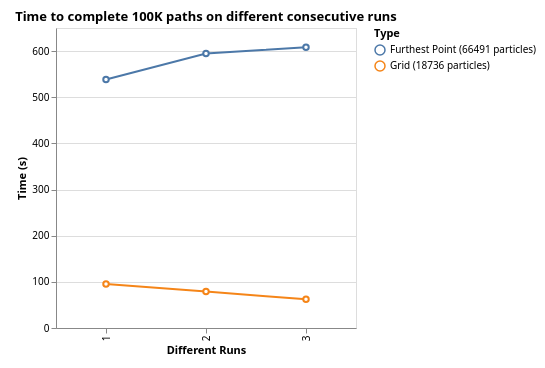
\includegraphics[width=0.41\linewidth]{Results/100KTime.png}}

    \caption{Time to complete of different consecutive runs with 10K 
    and 100K paths for run} 
    \label{fig:timeTestsBase}
\end{figure}

\subsubsection{Impact of Multi-Resolution in Computational Cost}

We have tested the base erosion algorithm applied on different 
multi-resolution methods, but we have not yet applied it 
to the high-resolution method without any kind of multi-resolution. 
During some test runs, we found that repeating an experiment 
like the one we just presented (running 100 thousand paths three times)
would be incredibly slow, so we decided to present two simpler comparisons 
to show the advantage of using the multi-resolution process. 

\vspace{10pt}

In the first experiment, we compared the results of the furthest point 
method with a downscale factor of 10 against the high-resolution using 
the terrain \textit{Aneto} with a resolution of 150x150 (the previously used 
197x199 resolution was too expensive), both executing 
100,000 paths. The furthest point method took 437 seconds (7 minutes and 17 seconds), 
while the high-resolution model took 1661 seconds (27 minutes and 41 seconds). 
Regarding the final results, the high-resolution terrain produced almost negligible 
erosion effects on the terrain, which implies that even more water paths 
are required to properly display erosion effects. These visual results 
can be seen in figure \ref{fig:highResVsLow}.

\vspace{10pt}

\begin{figure}
    \centering

    \subfigure[Results of 100,000 paths using the furthest point method for multi-resolution]{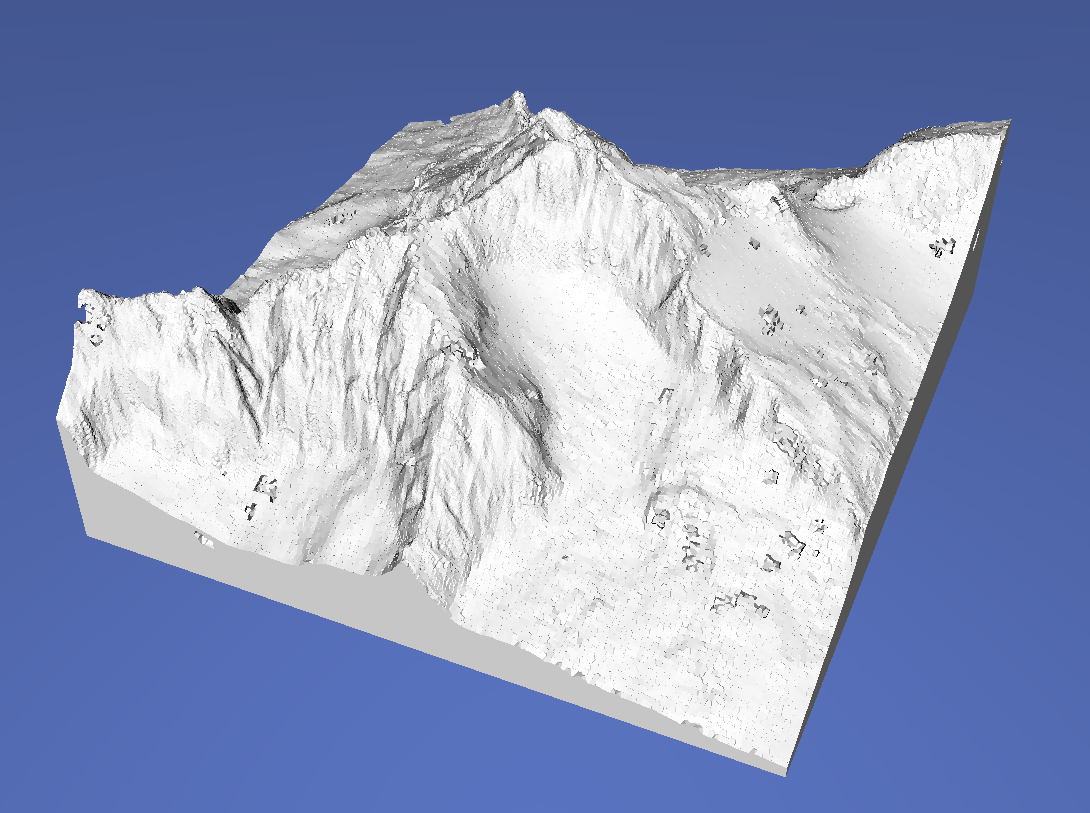
\includegraphics[width=0.38\linewidth]{Results/100KpathsAneto.png}
    }
    \hspace{20pt}    
    \subfigure[Results of 100,000 paths directly on the high resolution terrain]{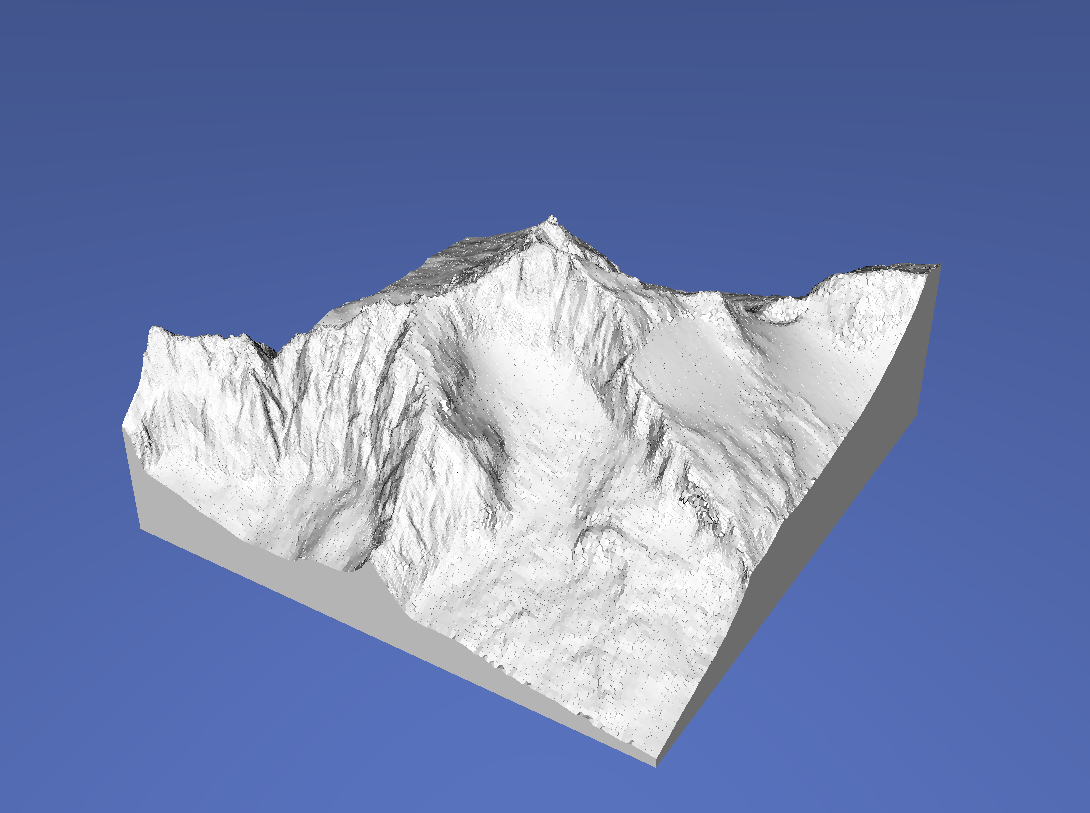
\includegraphics[width=0.38\linewidth]{Results/100KpathsAnetoHighres.png}}

    \caption{Results of 100,000 paths of the erosion simulation. Using a multi-resolution method 
    versus using the high resolution directly} 
    \label{fig:highResVsLow}
\end{figure}

The time that we save on the base erosion algorithm is highly significant, 
but having a multi-resolution method is even more essential if we want to use our 
mechanical model, as the difference is even greater. In order to show 
this difference, we initially wanted to test a single path 
in the high-resolution model using the same terrain we used for other 
experiments of the mechanical model (Aneto 50x50). We thought that a single 
path would show a huge difference in computation time, demonstrating 
the necessity for a multi-resolution method, but we could not even complete 
a single path (we timed out the experiment after an hour). This 
failure demonstrates the necessity of applying the multi-resolution method.

\vspace{10pt}

Despite this failure, we wanted to have some data to compare, so we tried 
again with a 25x25 Aneto terrain. In this case, the method that used 
multi-resolution took 587 ms for a single path, while the high-resolution 
model took 468149 ms (roughly 7 minutes and 48 seconds). This implies 
three orders of magnitude of difference between the two methods, and 
it seems to get even wider for higher terrain dimensions.
Using directly the high resolution for our tests would be basically 
unfeasible, so we completely discarded the idea of performing 
any comparison for other experiments.


\subsection{Mechanical Model Experimentation}
After experimenting with the base method, we are ready to test 
the algorithm using the mechanical model. The mechanical model is 
much more computationally expensive than the base algorithm due to the 
constant recomputation of the system of equations, so we need a simpler 
model to test. To perform all tests of our mechanical model, we used the \textit{Aneto} terrain with heightfield dimensions of
50x50 and a grid of 3x3x3 blocks for the low-resolution subsampling.

\subsubsection{Simulating Different Materials}

The number of parameters influencing our mechanical model is huge, and 
independently trying to tune every single one of them would be a challenging 
task. For that reason, we decided to first look in nature and try the 
mechanical properties of different rocks. We do not really need 
the parameters to exactly match the real ones, and we can work with 
an approximation, so we took the data from the website \cite{MakeitFrom} 
that lists some of the material properties of different materials. However,
that website does not list cohesion (c) and the coefficient of internal 
friction ($\varphi$), so we checked for those properties in other 
parts of the literature, like \cite{article}, \cite{article2}, and \cite{app15137481}.

\vspace{10pt}

Using the collected data on material properties, we did a test run for granite
just to check whether the model runs properly or not. In the test run,
we found that most links were, initially, over the shear stress limit, 
producing an initial crack propagation effect that destroyed a huge portion
of the terrain before starting the first path. For that reason, we decided 
to multiply by 10 the cohesion of all materials, and then we tried another test run 
with granite. In the second test run, some links broke initially due to 
tension, and a few cells were separated, but the initial damage was minor.
To avoid this initial damage we decided to increase the tensile strength 
by around 50\% on all materials. Figure \ref{fig:initialShearTension} shows 
the results of these two test runs.

\begin{figure}
    \centering

    \subfigure[Results using the initial cohesion, without modification]{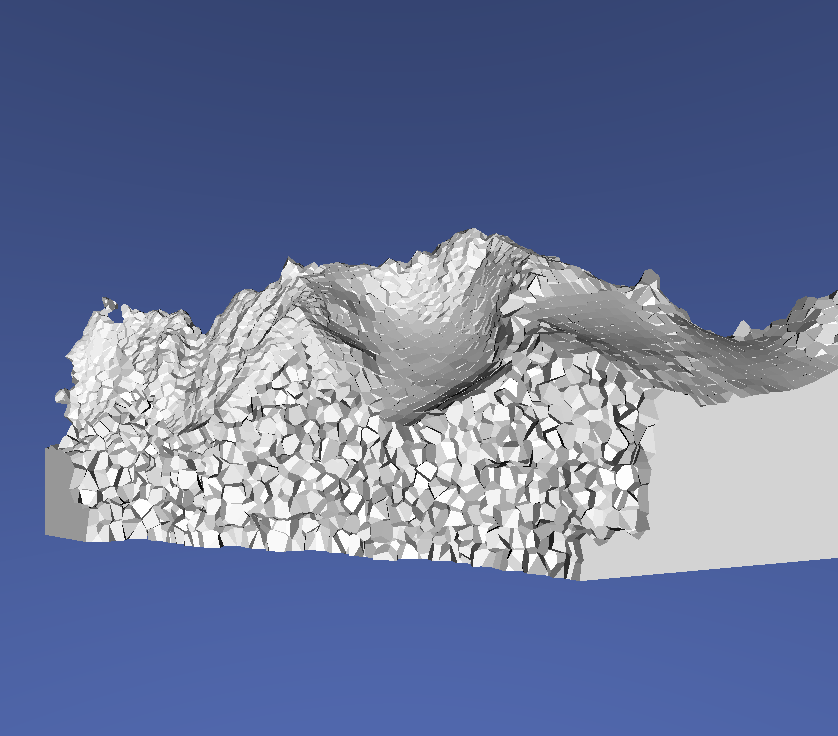
\includegraphics[width=0.38\linewidth]{Results/lowShearTest.png}
    }
    \hspace{20pt}    
    \subfigure[Minor damage initial damage on the terrain using the updated cohesion]{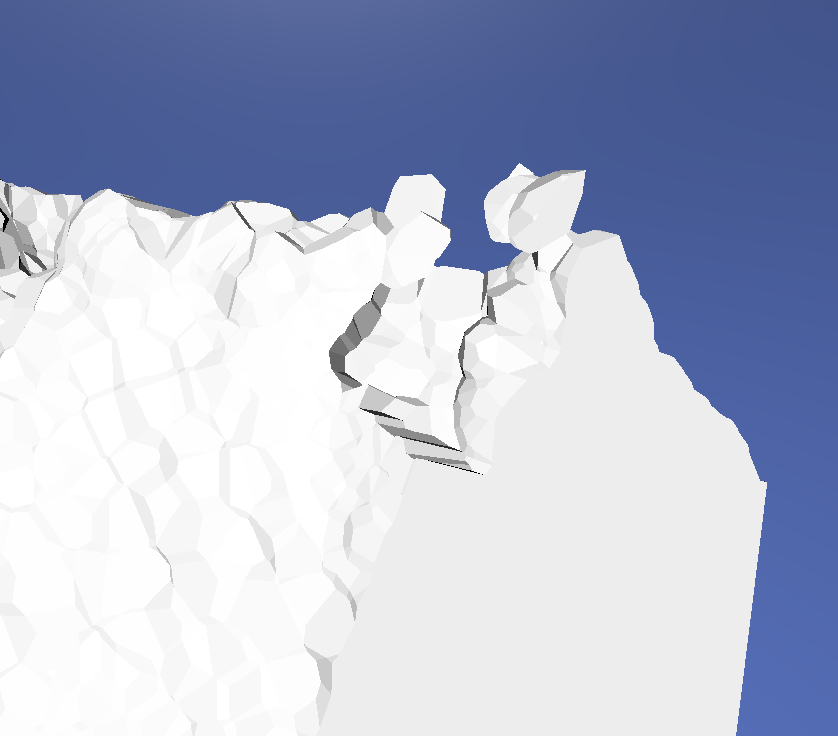
\includegraphics[width=0.38\linewidth]{Results/lowTensionTest.png}}

    \caption{Results of our test runs to tune the material properties} 
    \label{fig:initialShearTension}
\end{figure}

\vspace{10pt} 

\begin{table}[]
\centering
\begin{tabular}{|l|l|l|l|}
\hline
                             & Granite       & Marble        & Sandstone     \\ \hline
Density                      & $2650 \; kg/m^3$ & $2700 \; kg/m^3$ & $2600 \;  kg/m^3$ \\ \hline
Young's Modulus (E)          & 70 GPa          & 54 GPa          & 38 GPa          \\ \hline
Poisson's Ratio ($\upsilon$) & 0.255         & 0.2           & 0.25          \\ \hline
Tensile Strength ($T_{max}$)     & 60 MPa          & 12 MPa          & 6 MPa           \\ \hline
Compressive Strength (UCS)   & 2.2 GPa         & 540 MPa         & 120 MPa         \\ \hline
Cohesion (c)                 & 200 MPa         & 700 MPa         & 200 MPa         \\ \hline
$tan(\varphi)$                  & 0.267949      & 0.57735026    & 0.83909963   \\ \hline
\end{tabular}
\caption{Parameters of the tested materials. Some properties have 
been adjusted to our algorithm and might not fully represent the true 
material properties}
\label{tab:baseMaterialProperties}
\end{table}

After these test runs, we set the material properties of granite, marble, and 
sandstone to the values shown in table \ref{tab:baseMaterialProperties} and 
then started some experiments to compare the three. Granite showed 
pretty good results after simulating 100 paths (although we could not 
get to 200); the simulation took 
around 1000 seconds, and it produced a big hole in the middle of the 
mountain (somewhat resembling a volcano). Regarding the other two materials, 
marble showed some fractures after the initial stress computation (before 
generating any water path) and then completely collapsed after just 10 
paths, while sandstone did not even survive the initial stress computation. 
We based our parameters on the initial test runs on granite (which is 
the only one that survived a few paths), but it seems that our takeaways 
from the test runs were not really applicable to the other two materials.

\begin{figure}
    \centering

    \subfigure[Results of a granite Aneto after 100 water paths. 
    The terrain fully collapsed after just a few more paths]{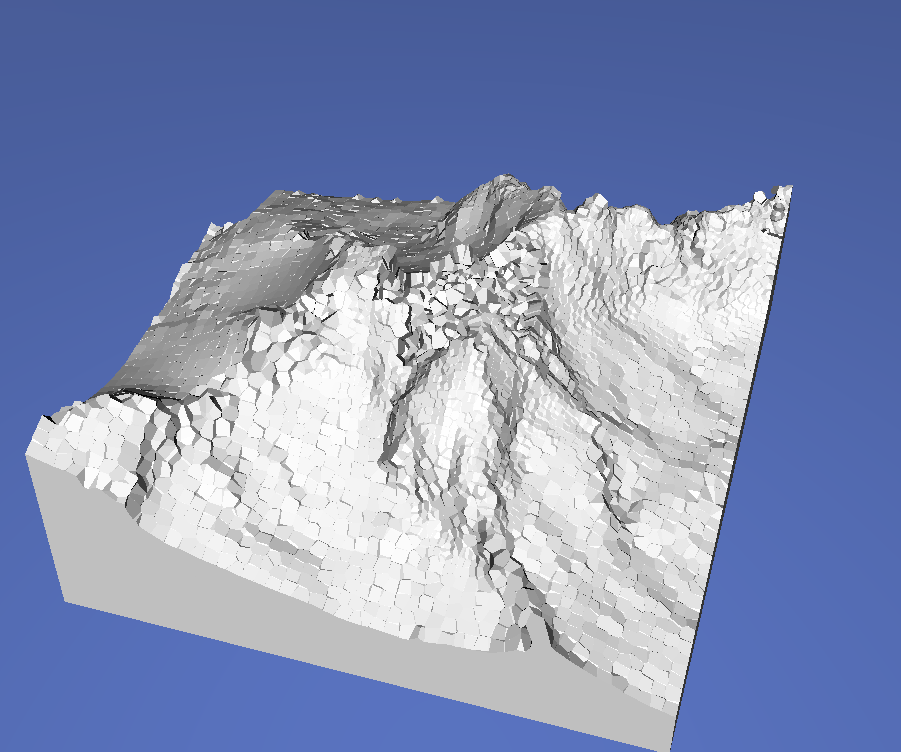
\includegraphics[width=0.4\linewidth]{Results/GraniteBase100.png}
    }
    \hspace{20pt}    
    \subfigure[Results of a marble Aneto after the initial stress computation (0 paths). The 
    terrain collapsed when we tried to simulate a few paths]{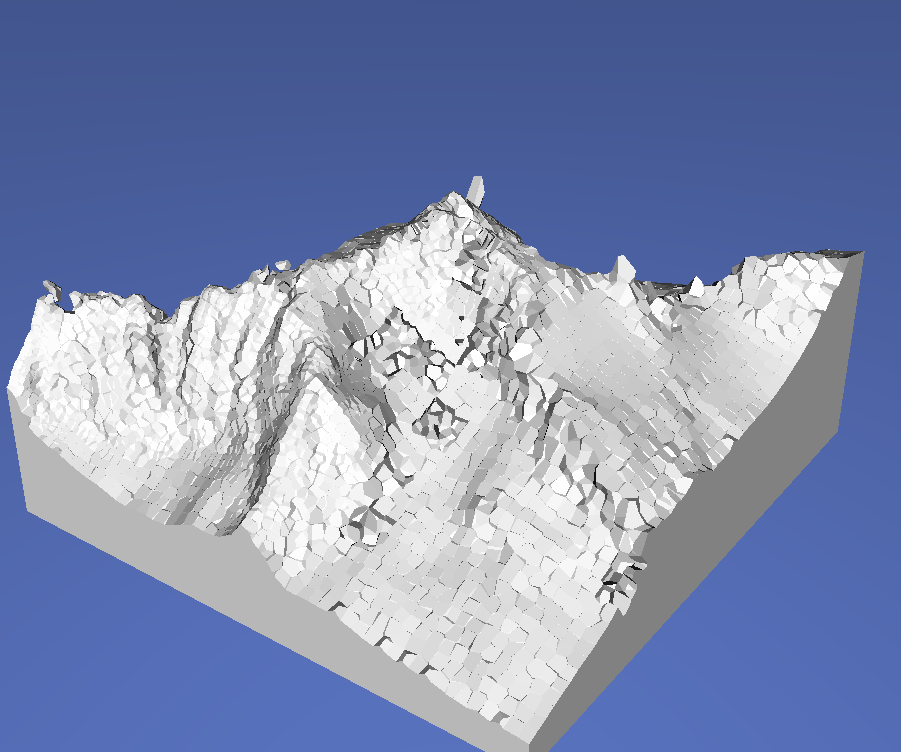
\includegraphics[width=0.4\linewidth]{Results/MarbleBase0.png}}

    \caption{Results of our experiments with different materials, just 
    before the terrains fully collapsed. Granite 
    sill retained some stability after 100 water paths, but marble collapsed 
    after less than 10} 
    \label{fig:initialMaterials}
\end{figure}

\subsubsection{Reinforced Materials}

In response to the poor results of the first experiments with different 
materials, we decided to reinforce their tensile strength so they 
can resist at least a few water paths. We decided to adjust 
just the tensile strength because most links were breaking due to tension 
and not due to shear or compression stresses. To differentiate these 
modified materials from the base materials that we tried previously, 
we decided to call them \textit{reinforced materials}, with properties 
shown in table \ref{tab:reinforcedMaterials}.


\begin{table}[]
\centering
\begin{tabular}{|l|l|l|l|}
\hline
                             & Reinforced Granite       & Reinforced Marble        & Reinforced Sandstone     \\ \hline
Density                      & $2650 \; kg/m^3$ & $2700 \; kg/m^3$ & $2600 \;  kg/m^3$ \\ \hline
Young's Modulus (E)          & 70 GPa          & 54 GPa          & 38 GPa          \\ \hline
Poisson's Ratio ($\upsilon$) & 0.255         & 0.2           & 0.25          \\ \hline
Tensile Strength ($T_{max}$)     & 390 MPa         & 120 MPa          & 60 MPa           \\ \hline
Compressive Strength (UCS)   & 2.2 GPa         & 540 MPa         & 120 MPa         \\ \hline
Cohesion (c)                 & 200 MPa         & 700 MPa         & 200 MPa         \\ \hline
$tan(\varphi)$                  & 0.267949      & 0.57735026    & 0.83909963   \\ \hline
\end{tabular}
\caption{Parameters that we used as our \textit{reinforced} materials}
\label{tab:reinforcedMaterials}
\end{table}

\vspace{10pt}

Using these new reinforced materials, our experiments looked much better, and 
we were able to compare the effect of changing the material on the 
overall results. After 400 water paths on each material, granite 
produced multiple holes but remaind fairly stable; sandstone had a wide 
portion completely destroyed; and, finally, 
marble seemed the most resistant, producing thin and shallow holes. 
The comparison between the different materials can be seen in figure \ref{fig:meterialComparison}

\begin{figure}
    \centering

    \subfigure[Eroion simulation after 400 paths on reinforced granite. Overview]{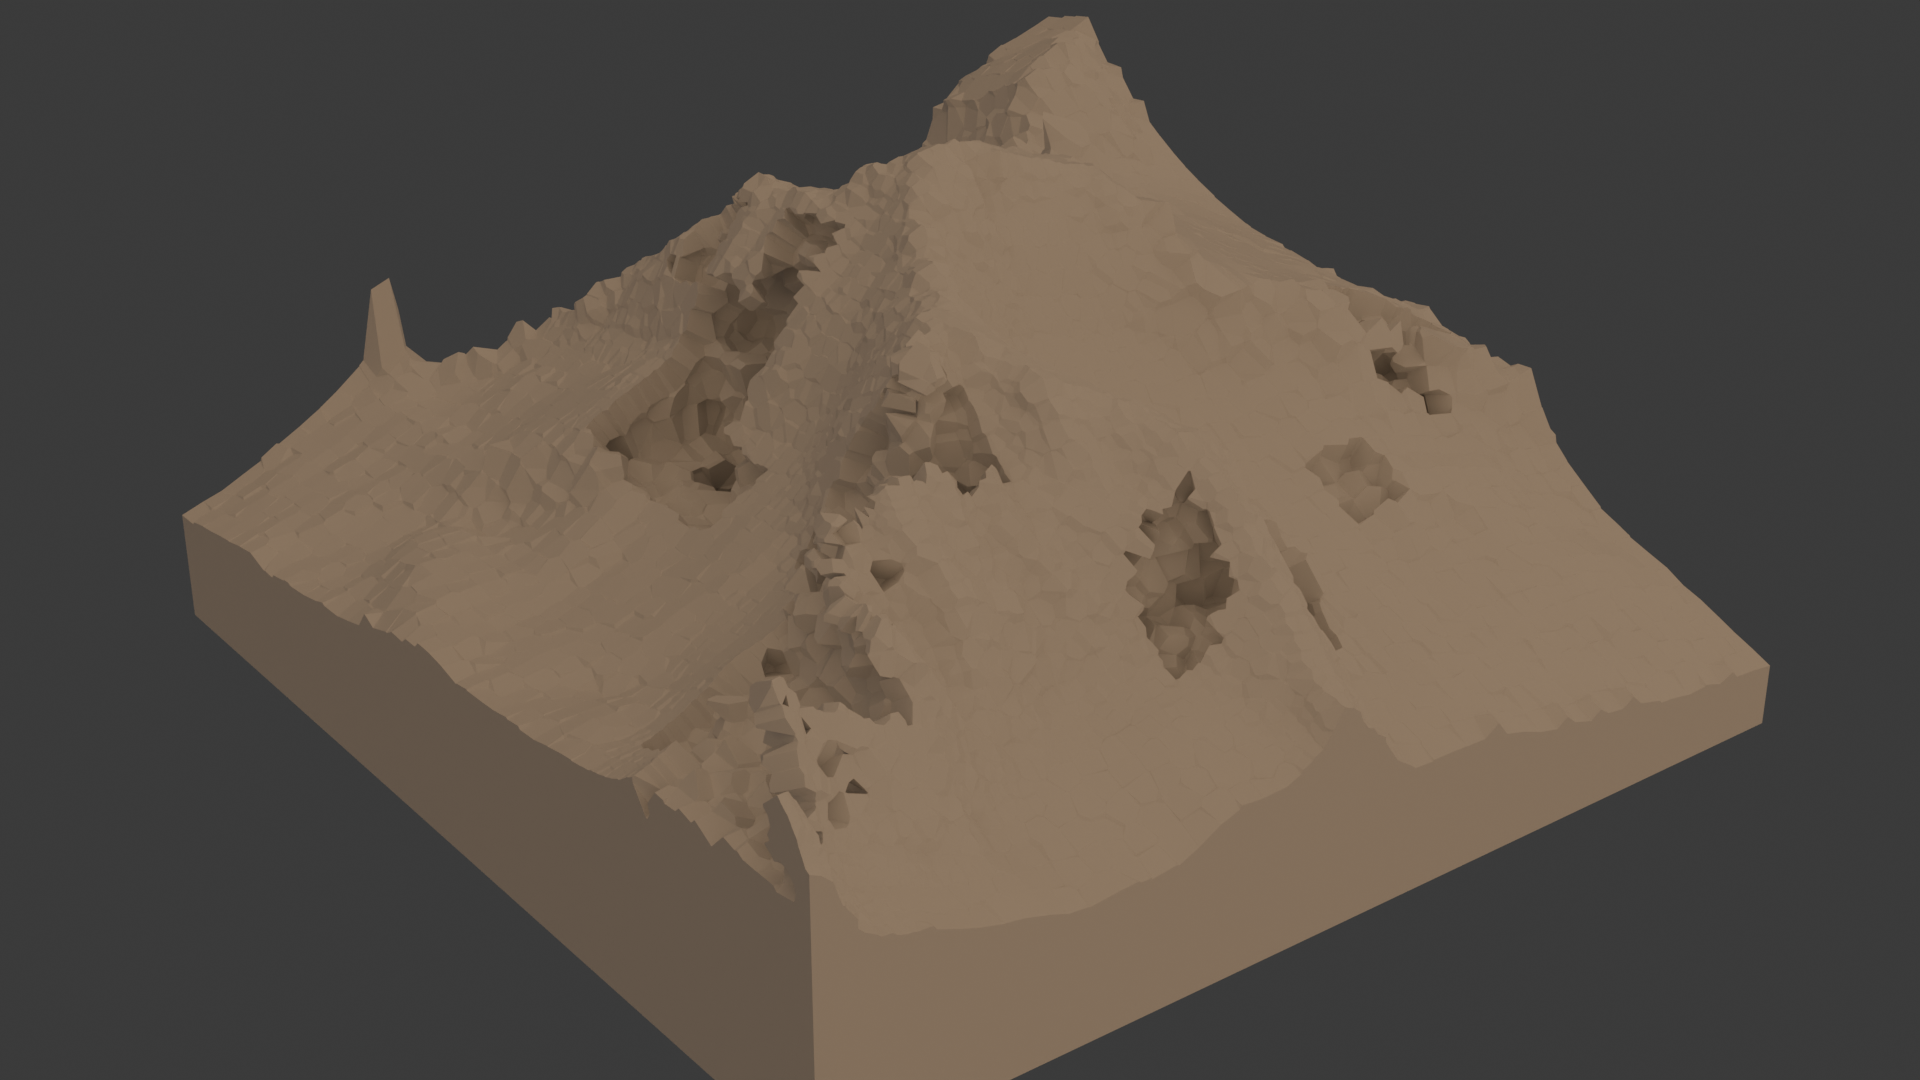
\includegraphics[width=0.48\linewidth]{Results/Renders/gramnite400Overview.png}
    }
    \hspace{5pt}
    \subfigure[Eroion simulation after 400 paths on reinforced granite. Zoomed]{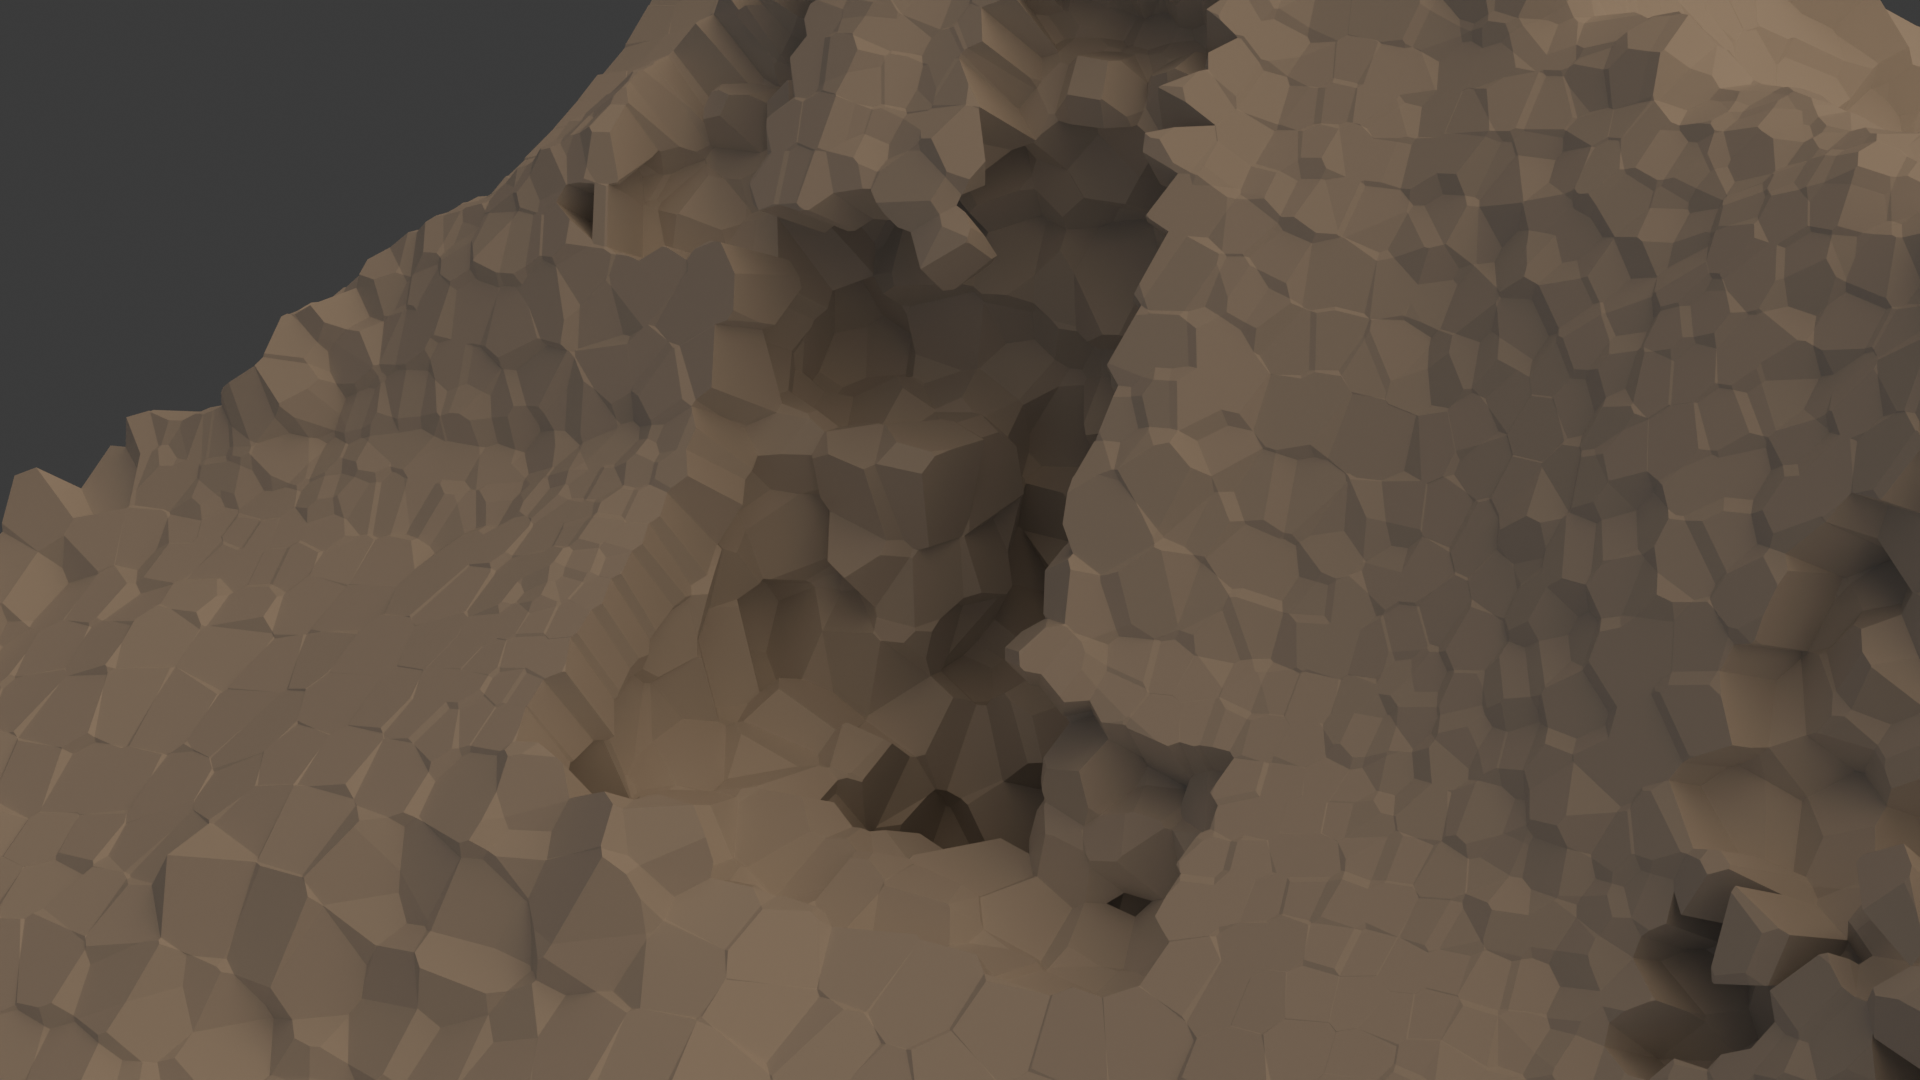
\includegraphics[width=0.48\linewidth]{Results/Renders/graniteDetail.png}}
    \hfill
    \subfigure[Eroion simulation after 400 paths on reinforced marble. Overview]{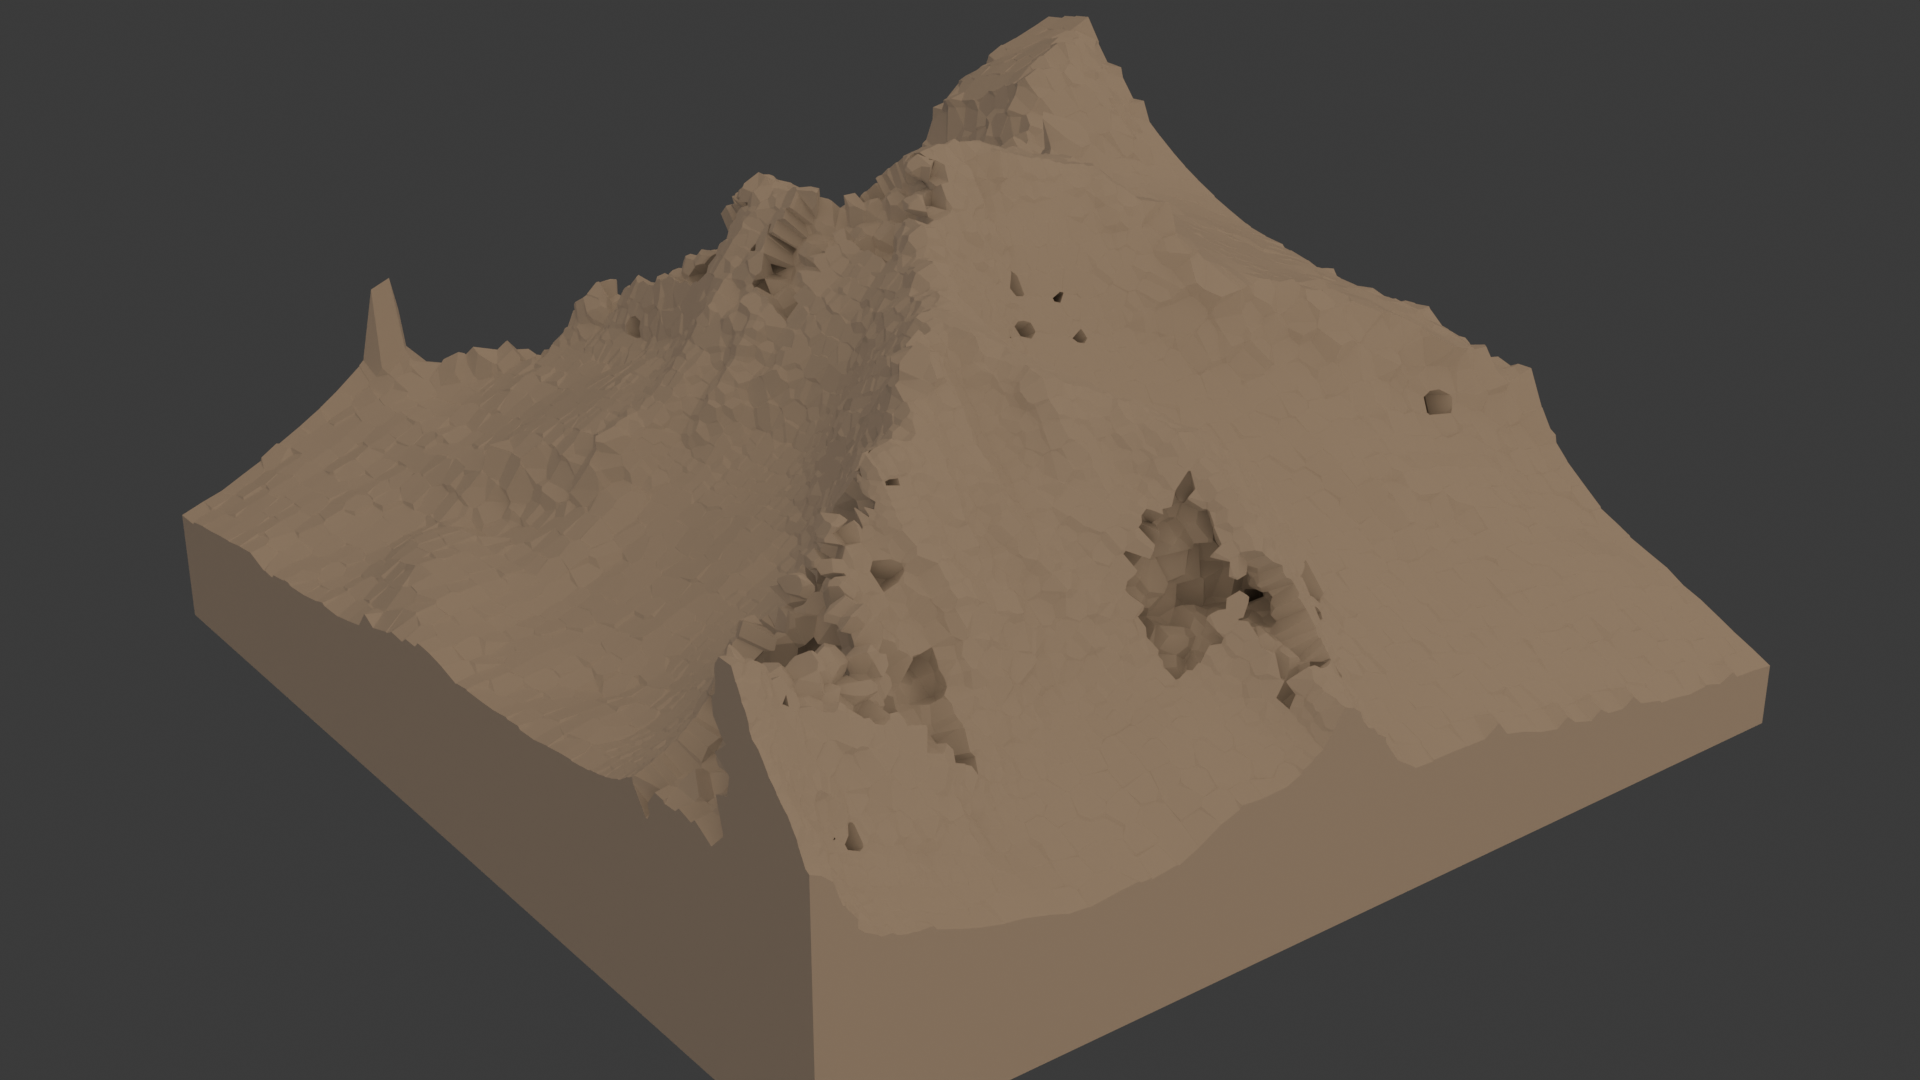
\includegraphics[width=0.48\linewidth]{Results/Renders/marble400Overview.png}}
    \hspace{5pt}
    \subfigure[Eroion simulation after 400 paths on reinforced marble. Zoomed]{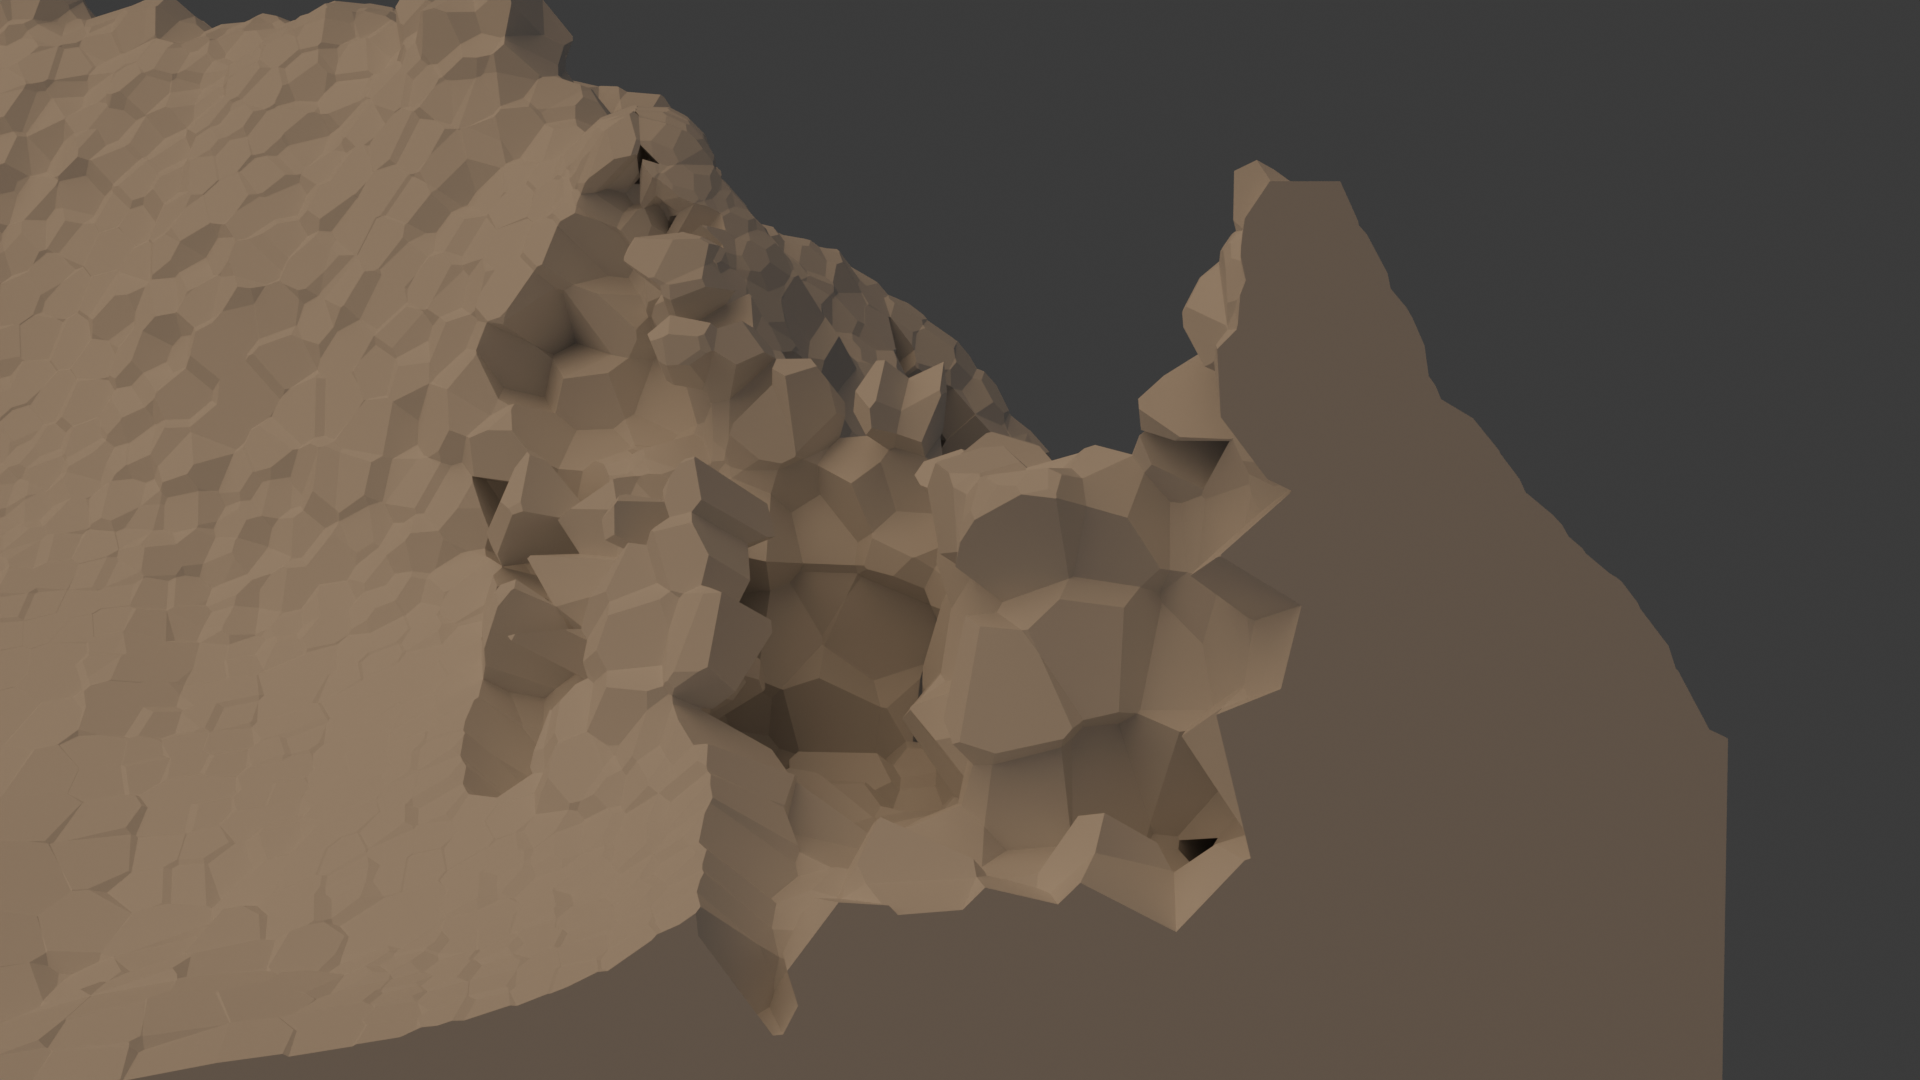
\includegraphics[width=0.48\linewidth]{Results/Renders/marbleDetail.png}}
    \hfill
    \subfigure[Eroion simulation after 400 paths on reinforced sandstone. Overview]{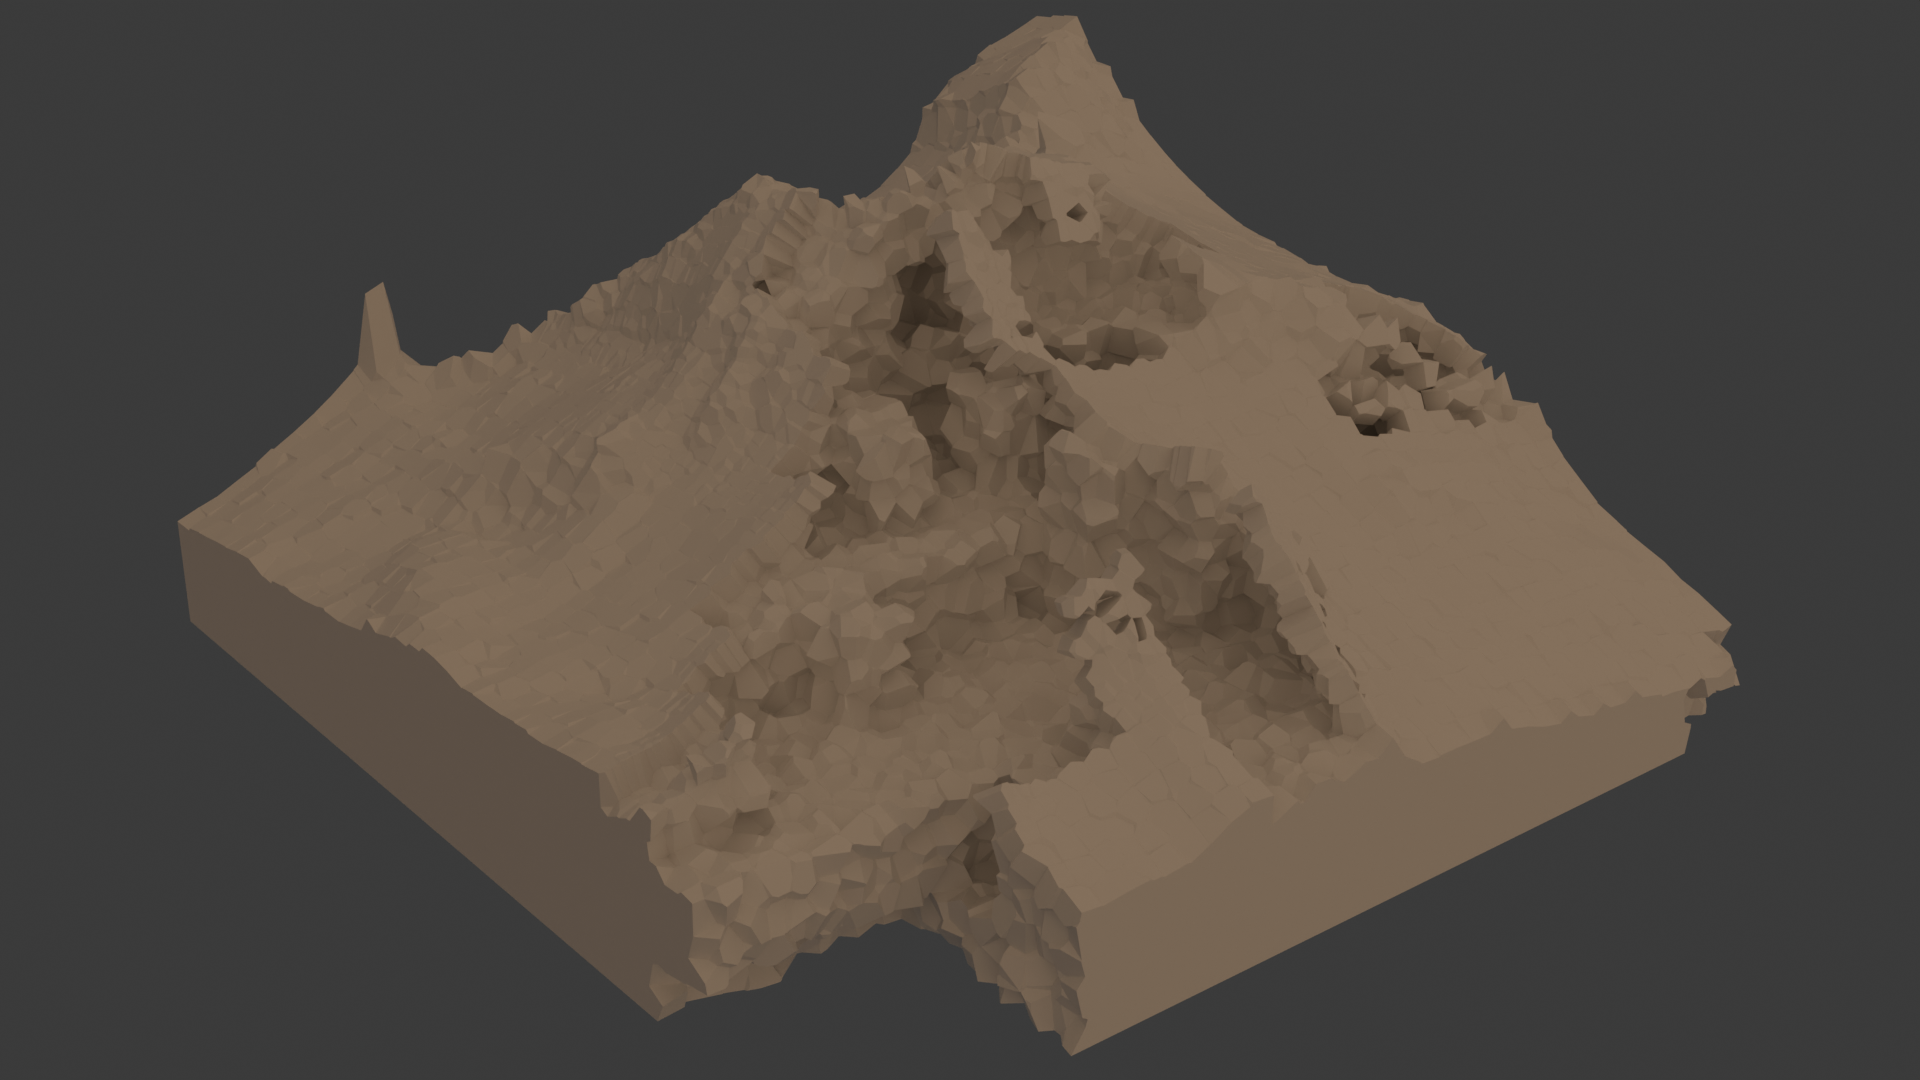
\includegraphics[width=0.48\linewidth]{Results/Renders/sandstone400Overview_4.png}}
    \hspace{5pt}
    \subfigure[Eroion simulation after 400 paths on reinforced sandstone. Zoomed]{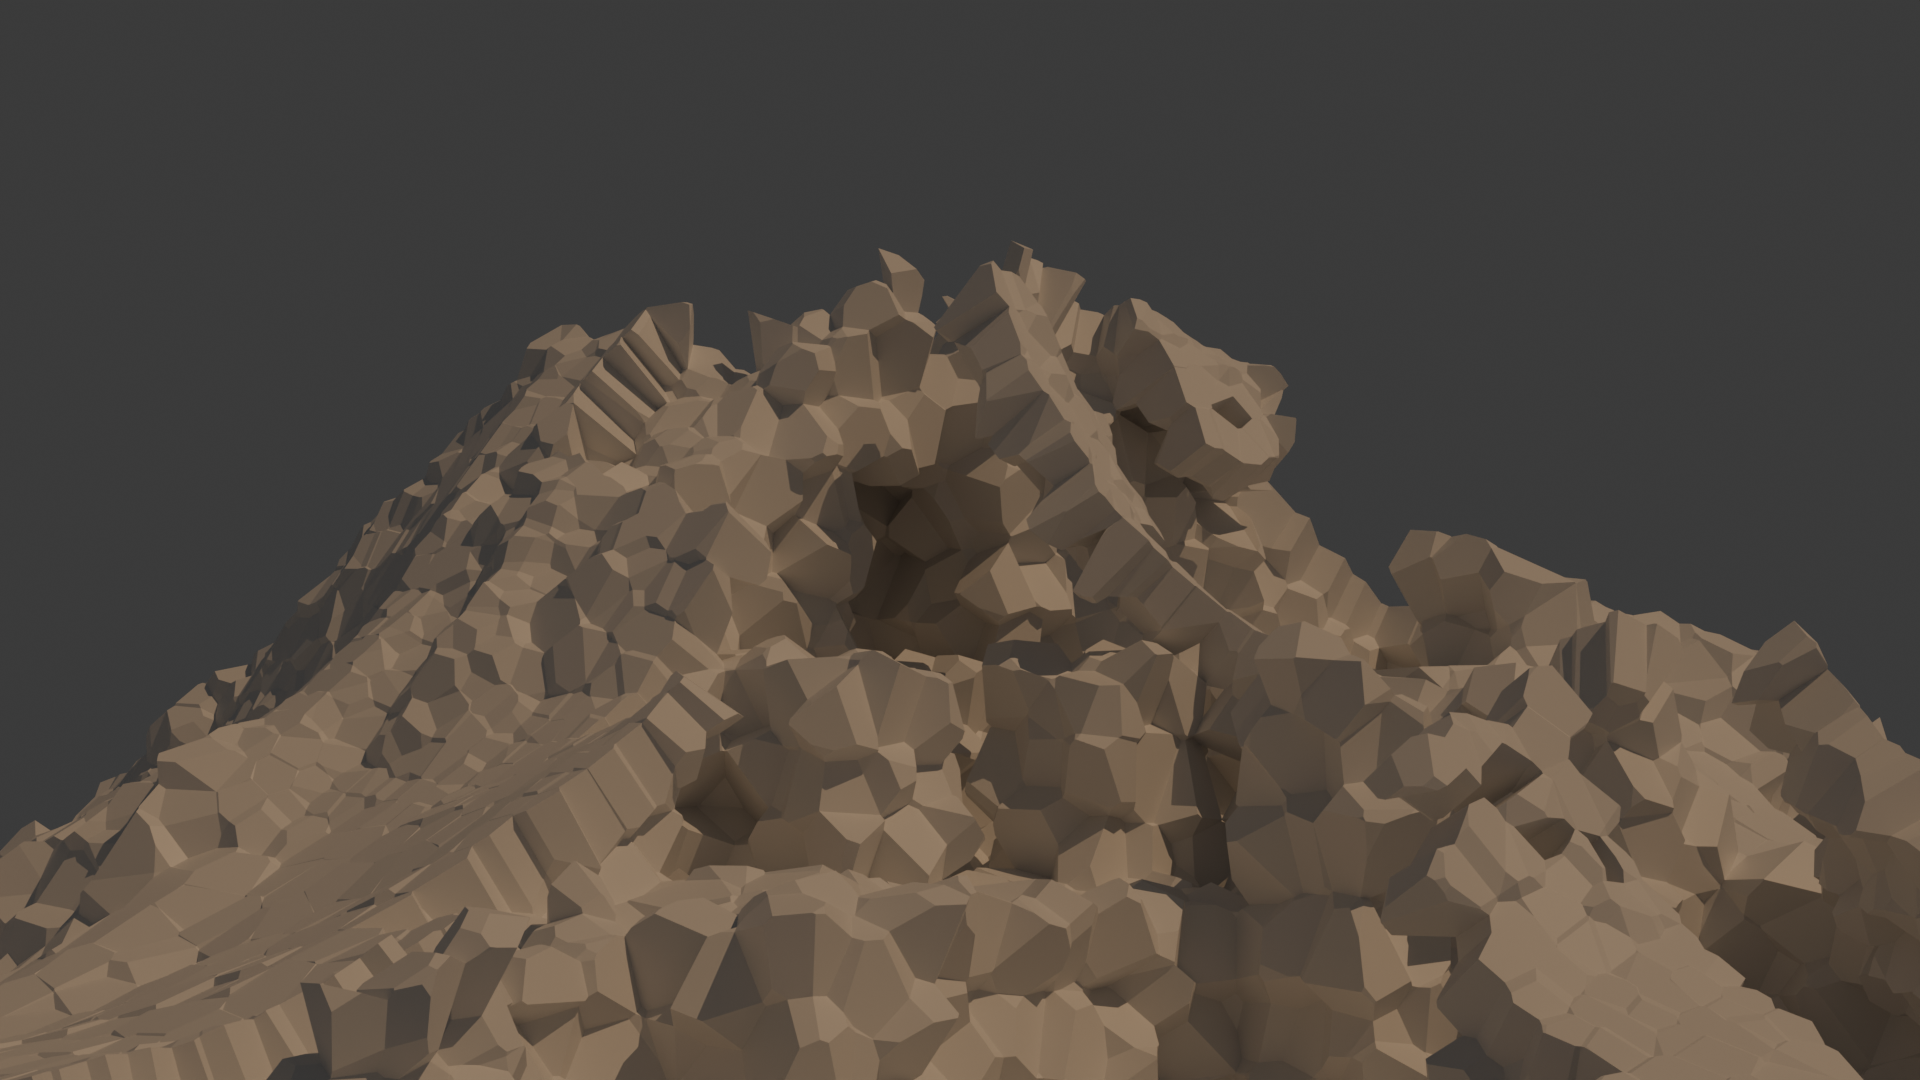
\includegraphics[width=0.48\linewidth]{Results/Renders/sandstoneDetail.png}}


    \caption{Erosion simulation after 400 paths on different reinforced materials.
    All images have been rendered on Blender using the exported eroded terrain 
    from our application} 
    \label{fig:meterialComparison}
\end{figure}


%\subsubsection{Failure Parameter Tunning}
\subsubsection{Computational Time Results}

During all of our experiments, we also collected data on their time 
to compute. Unlike the base algorithm, separating parts is not the 
most expensive task of this method, as the most expensive one is 
recomputing the system, which happens every time a link is broken. Link 
removal is much whole more common than cell removals, so they are expected to 
appear through each state of the erosion simulation process. Technically, 
the probability of a link breaking depends on the stress of the system, 
but the relationship between the number of paths executed and the 
probability of a link breaking is not that simple to compute. The only clear 
relationship between the amount of paths already computed and the 
cost of the next path is the number of remaining cells; the fewer 
cells there are, the cheaper it is to compute the state of the system.

\vspace{10pt}

Regarding the computational cost, we performed an experiment 
using reinforced sandstone that provided really useful information. 
We tried 15 consecutive rounds of 25 paths each (for a total of 375 paths) 
measuring the time they took to compute and the remaining cells after 
the computation. In figure \ref{fig:computationTimePerPath} we can see 
that the average time to compute a water path varies a lot for each 
consecutive round but with a downward trend in the last four 
paths. We can relate this downward trend to the number of cells 
seen in figure \ref{fig:cellNum}: the last four rounds have a marked 
decrease in the number of cells, so cheaper computations are expected.

\begin{figure}
    \centering 
    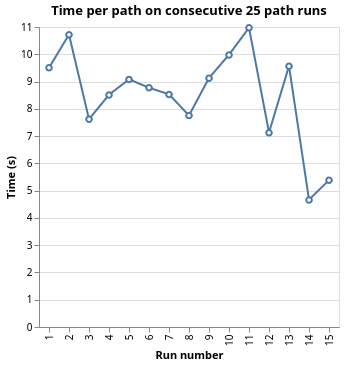
\includegraphics[scale = 0.35]{Results/timePerPathSandstone.png}
    \caption{Time per path on different consecutive 25 path runs using 
    the reinforced sandstone material}
    \label{fig:computationTimePerPath}
\end{figure}
\begin{figure}
    \centering 
    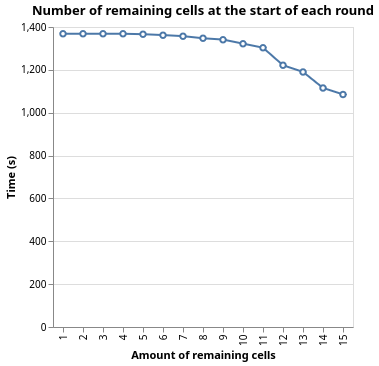
\includegraphics[scale = 0.35]{Results/cellsPerRound.png}
    \caption{Remaining cells at the begining of each consecutive round 
    of 25 paths}
    \label{fig:cellNum}
\end{figure}
\subsection{Method Comparison}

Finally, after conducting all experiments, we are ready to compare 
the results of the erosion process using the base method and the 
method including the mechanical model. In order to do a fair comparison, 
we compared the results on the \textit{Aneto} terrain using a 50x50 grid 
for the heightfield and a 3x3x3 block grid to perform subsampling.

\vspace{10pt}

The first important difference is the computational cost. Different 
experiments on different materials using the mechanical model required 
multiple seconds per path, while our test on the same 
model using the base method took only tens of microseconds. Fortunately, 
our improved method required fewer paths to erode the model: we could 
appreciate the results with just a hundred paths, while the base method 
required at least a few thousand. This difference in the number of paths 
required to erode helps reduce the computational cost of the 
improved method (as we do not need to perform that many paths).

\vspace{10pt}

After going over the cost comparison, we have to mention the most important
part: the results of the erosion simulation. The main problem with 
the base algorithm is that it generates multiple structures that are 
almost floating, only connected to the terrain through a thin chain 
of rocks. On the other hand, our improved method does not produce these 
almost floating chunks, and the resulting terrain appears to be much 
more physically stable. 

\begin{figure}
    \centering

    \subfigure[Aneto terrain after applying the base algorithm (without mechanical model).
    A big portion of the bottom of the terrain is removed but parts of the surface 
    still survive almost floating]{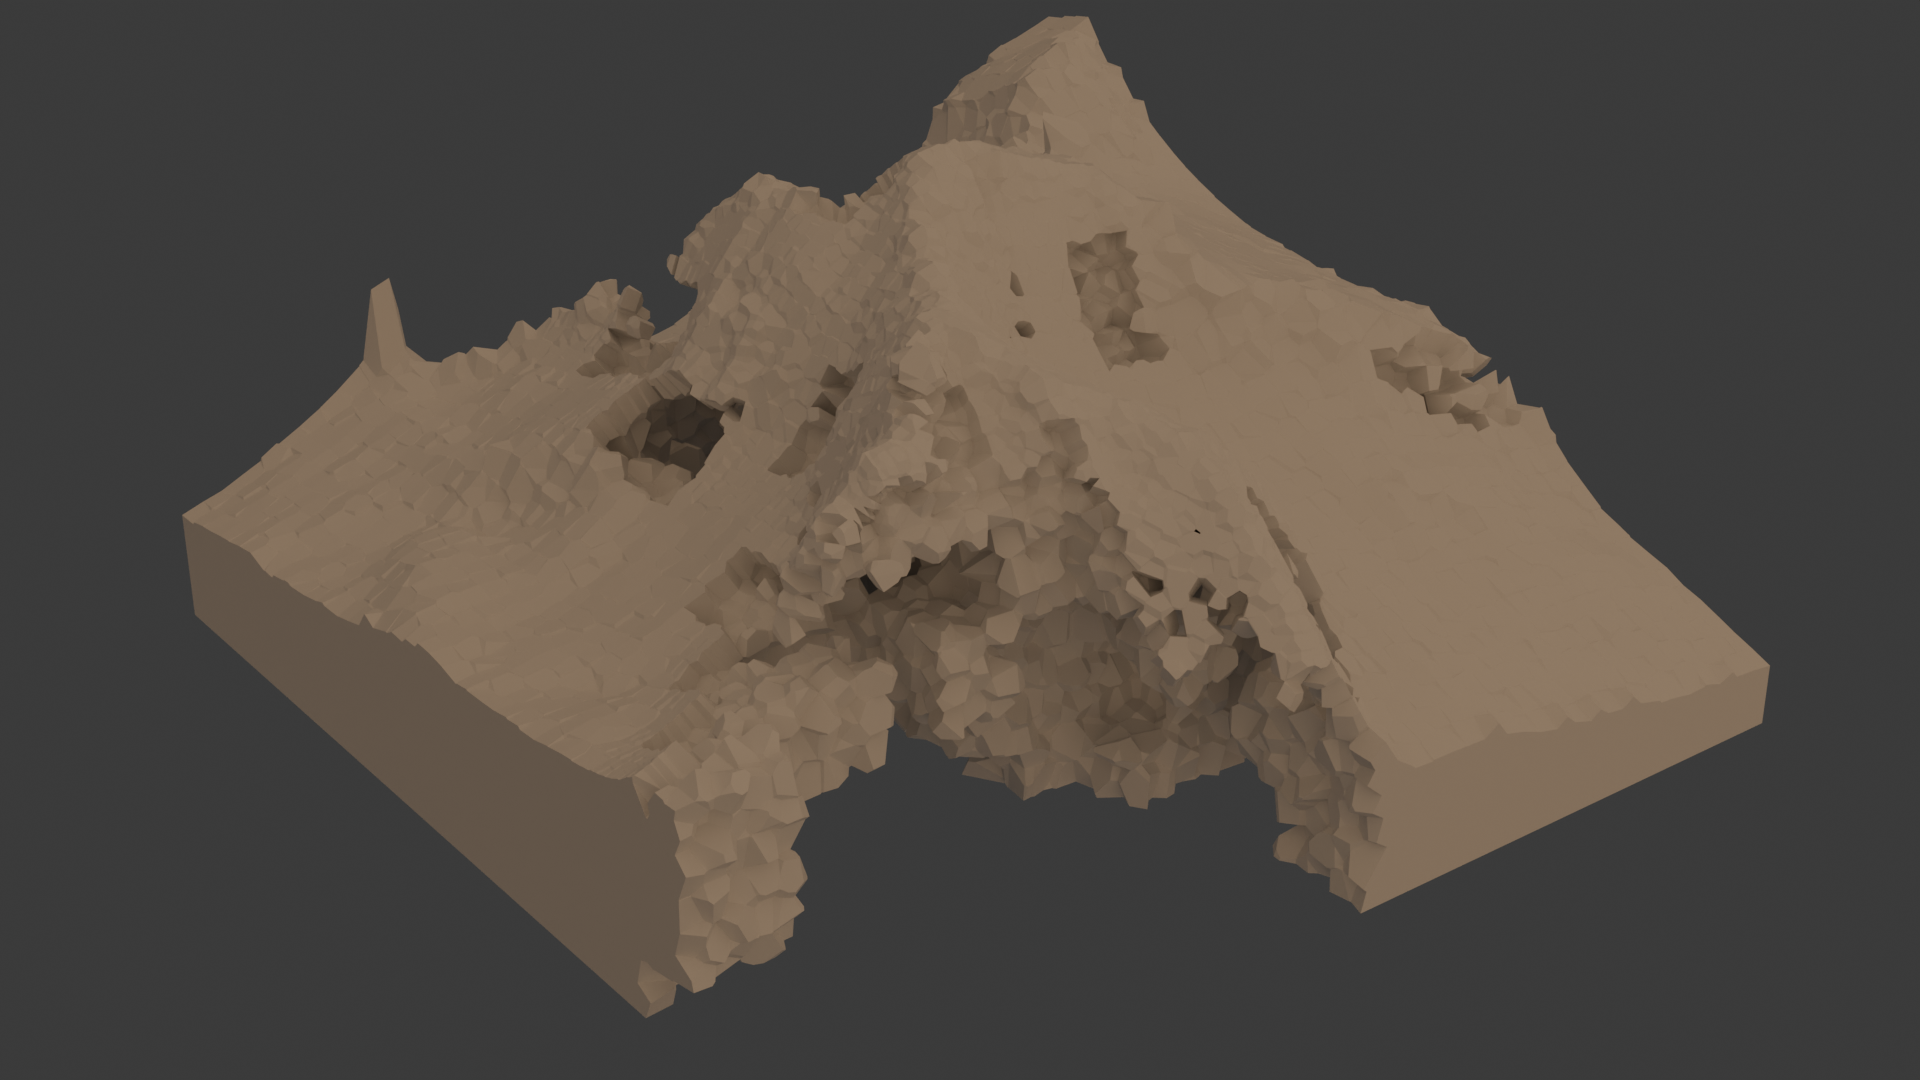
\includegraphics[width=0.45\linewidth]{Results/Renders/baseErosionOverview1.png}
    }
    \hspace{20pt}    
    \subfigure[Aneto mountain after applying the mechanical model using our reinforced sandstone.
    In this case the surface of the mountain has mostly fallen along the bottom section of the terrain]{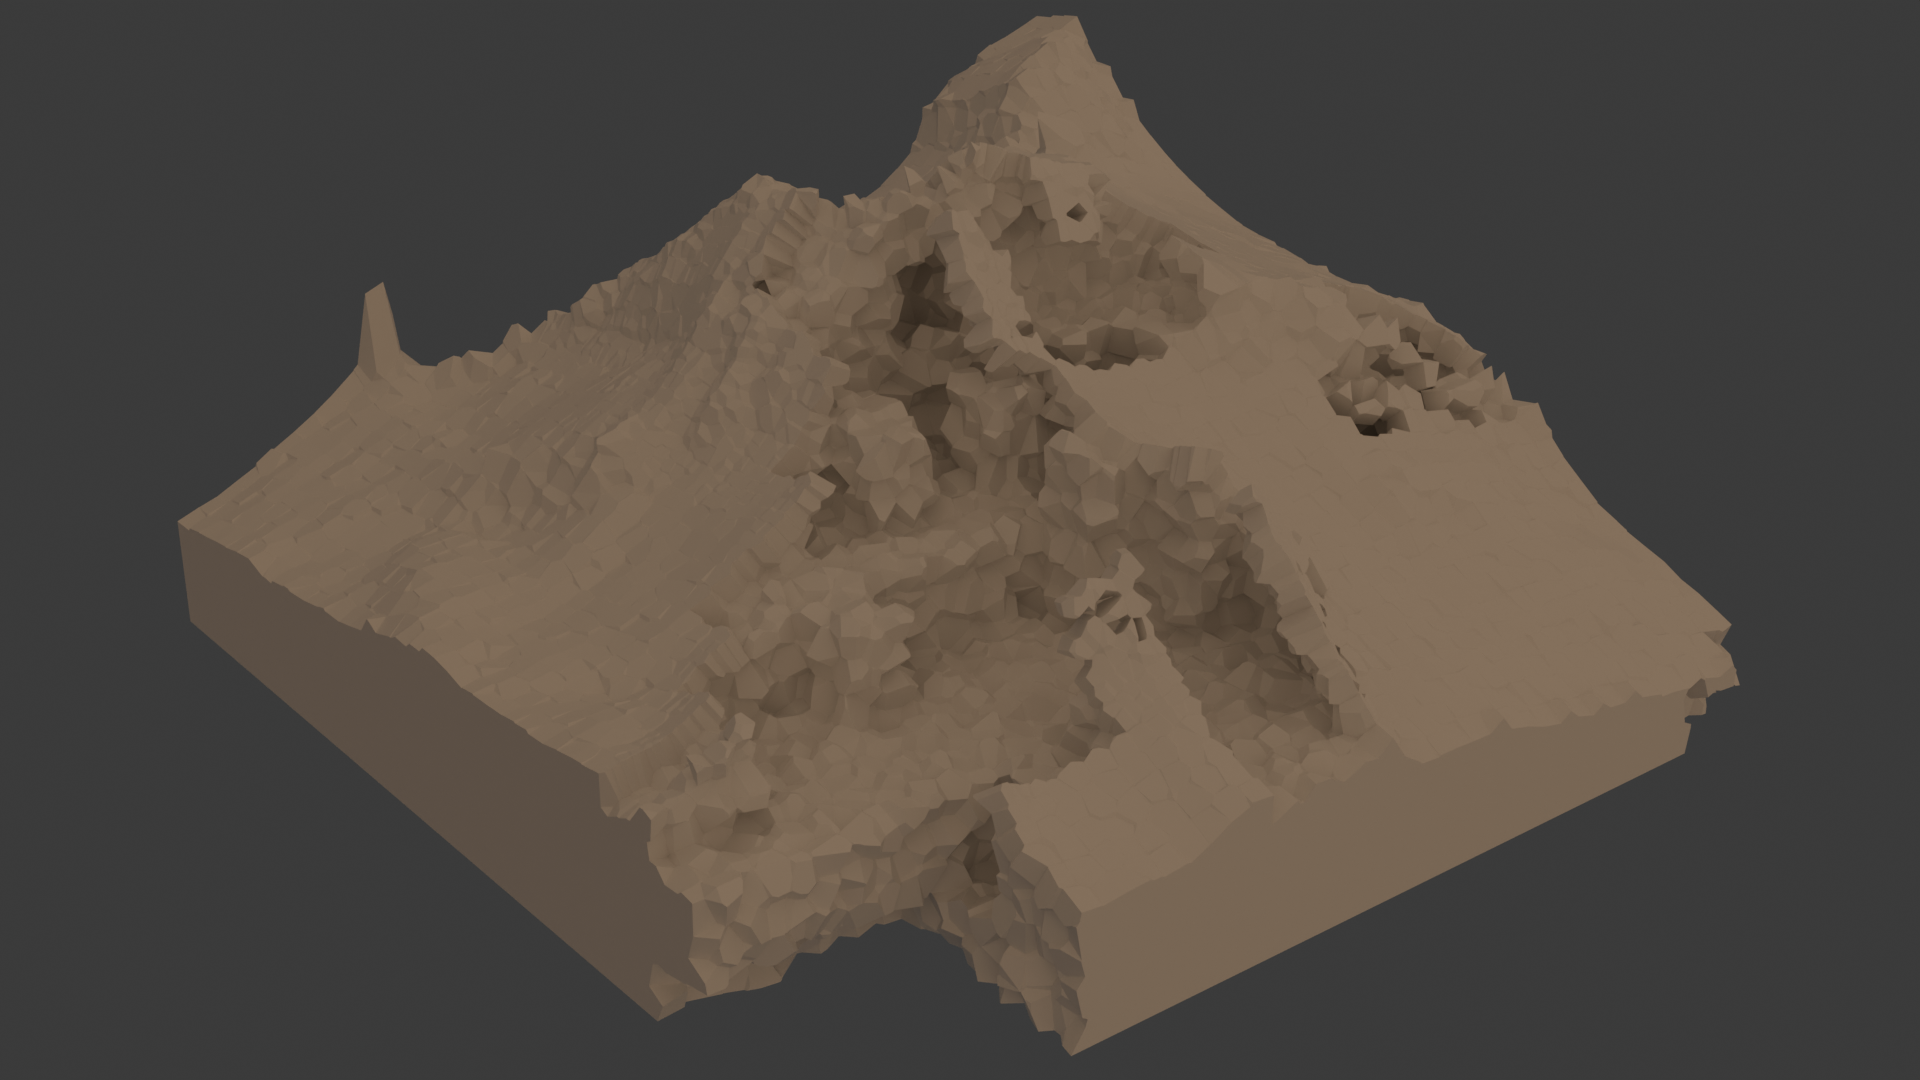
\includegraphics[width=0.45\linewidth]{Results/Renders/sandstone400Overview_4.png}}

    \caption{Figure comparing the base algorithm with our improved algorithm using 
    reinforced sandstone as a material. All images have been rendered using 
    Blender after exporting the eroded terrain} 
    \label{fig:baseVsMech}
\end{figure}

